\documentclass[twoside]{book}

% Packages required by doxygen
\usepackage{calc}
\usepackage{doxygen}
\usepackage{graphicx}
\usepackage[utf8]{inputenc}
\usepackage{makeidx}
\usepackage{multicol}
\usepackage{multirow}
\usepackage{textcomp}
\usepackage[table]{xcolor}

% Font selection
\usepackage[T1]{fontenc}
\usepackage{mathptmx}
\usepackage[scaled=.90]{helvet}
\usepackage{courier}
\usepackage{amssymb}
\usepackage{sectsty}
\renewcommand{\familydefault}{\sfdefault}
\allsectionsfont{%
  \fontseries{bc}\selectfont%
  \color{darkgray}%
}
\renewcommand{\DoxyLabelFont}{%
  \fontseries{bc}\selectfont%
  \color{darkgray}%
}

% Page & text layout
\usepackage{geometry}
\geometry{%
  a4paper,%
  top=2.5cm,%
  bottom=2.5cm,%
  left=2.5cm,%
  right=2.5cm%
}
\tolerance=750
\hfuzz=15pt
\hbadness=750
\setlength{\emergencystretch}{15pt}
\setlength{\parindent}{0cm}
\setlength{\parskip}{0.2cm}
\makeatletter
\renewcommand{\paragraph}{%
  \@startsection{paragraph}{4}{0ex}{-1.0ex}{1.0ex}{%
    \normalfont\normalsize\bfseries\SS@parafont%
  }%
}
\renewcommand{\subparagraph}{%
  \@startsection{subparagraph}{5}{0ex}{-1.0ex}{1.0ex}{%
    \normalfont\normalsize\bfseries\SS@subparafont%
  }%
}
\makeatother

% Headers & footers
\usepackage{fancyhdr}
\pagestyle{fancyplain}
\fancyhead[LE]{\fancyplain{}{\bfseries\thepage}}
\fancyhead[CE]{\fancyplain{}{}}
\fancyhead[RE]{\fancyplain{}{\bfseries\leftmark}}
\fancyhead[LO]{\fancyplain{}{\bfseries\rightmark}}
\fancyhead[CO]{\fancyplain{}{}}
\fancyhead[RO]{\fancyplain{}{\bfseries\thepage}}
\fancyfoot[LE]{\fancyplain{}{}}
\fancyfoot[CE]{\fancyplain{}{}}
\fancyfoot[RE]{\fancyplain{}{\bfseries\scriptsize Generated on Fri Dec 4 2015 12\-:58\-:39 for R\-A\-P\-P Platform Tests -\/ Knowrob Wrapper by Doxygen }}
\fancyfoot[LO]{\fancyplain{}{\bfseries\scriptsize Generated on Fri Dec 4 2015 12\-:58\-:39 for R\-A\-P\-P Platform Tests -\/ Knowrob Wrapper by Doxygen }}
\fancyfoot[CO]{\fancyplain{}{}}
\fancyfoot[RO]{\fancyplain{}{}}
\renewcommand{\footrulewidth}{0.4pt}
\renewcommand{\chaptermark}[1]{%
  \markboth{#1}{}%
}
\renewcommand{\sectionmark}[1]{%
  \markright{\thesection\ #1}%
}

% Indices & bibliography
\usepackage{natbib}
\usepackage[titles]{tocloft}
\setcounter{tocdepth}{3}
\setcounter{secnumdepth}{5}
\makeindex

% Hyperlinks (required, but should be loaded last)
\usepackage{ifpdf}
\ifpdf
  \usepackage[pdftex,pagebackref=true]{hyperref}
\else
  \usepackage[ps2pdf,pagebackref=true]{hyperref}
\fi
\hypersetup{%
  colorlinks=true,%
  linkcolor=blue,%
  citecolor=blue,%
  unicode%
}

% Custom commands
\newcommand{\clearemptydoublepage}{%
  \newpage{\pagestyle{empty}\cleardoublepage}%
}


%===== C O N T E N T S =====

\begin{document}

% Titlepage & ToC
\hypersetup{pageanchor=false}
\pagenumbering{roman}
\begin{titlepage}
\vspace*{7cm}
\begin{center}%
{\Large R\-A\-P\-P Platform Tests -\/ Knowrob Wrapper }\\
\vspace*{1cm}
{\large Generated by Doxygen 1.8.6}\\
\vspace*{0.5cm}
{\small Fri Dec 4 2015 12:58:39}\\
\end{center}
\end{titlepage}
\clearemptydoublepage
\tableofcontents
\clearemptydoublepage
\pagenumbering{arabic}
\hypersetup{pageanchor=true}

%--- Begin generated contents ---
\chapter{Namespace Index}
\section{Namespace List}
Here is a list of all namespaces with brief descriptions\-:\begin{DoxyCompactList}
\item\contentsline{section}{\hyperlink{namespacecognitive__exercise}{cognitive\-\_\-exercise} }{\pageref{namespacecognitive__exercise}}{}
\item\contentsline{section}{\hyperlink{namespacecognitive__exercise__main}{cognitive\-\_\-exercise\-\_\-main} }{\pageref{namespacecognitive__exercise__main}}{}
\item\contentsline{section}{\hyperlink{namespacemysql__wrapper}{mysql\-\_\-wrapper} }{\pageref{namespacemysql__wrapper}}{}
\item\contentsline{section}{\hyperlink{namespacemysql__wrapper__main}{mysql\-\_\-wrapper\-\_\-main} }{\pageref{namespacemysql__wrapper__main}}{}
\item\contentsline{section}{\hyperlink{namespacerapp__audio__processing}{rapp\-\_\-audio\-\_\-processing} }{\pageref{namespacerapp__audio__processing}}{}
\item\contentsline{section}{\hyperlink{namespacerapp__audio__processing_1_1rapp__audio__processing}{rapp\-\_\-audio\-\_\-processing.\-rapp\-\_\-audio\-\_\-processing} }{\pageref{namespacerapp__audio__processing_1_1rapp__audio__processing}}{}
\item\contentsline{section}{\hyperlink{namespacerapp__audio__processing_1_1rapp__detect__silence}{rapp\-\_\-audio\-\_\-processing.\-rapp\-\_\-detect\-\_\-silence} }{\pageref{namespacerapp__audio__processing_1_1rapp__detect__silence}}{}
\item\contentsline{section}{\hyperlink{namespacerapp__audio__processing_1_1rapp__energy__denoise}{rapp\-\_\-audio\-\_\-processing.\-rapp\-\_\-energy\-\_\-denoise} }{\pageref{namespacerapp__audio__processing_1_1rapp__energy__denoise}}{}
\item\contentsline{section}{\hyperlink{namespacerapp__audio__processing_1_1rapp__set__noise__profile}{rapp\-\_\-audio\-\_\-processing.\-rapp\-\_\-set\-\_\-noise\-\_\-profile} }{\pageref{namespacerapp__audio__processing_1_1rapp__set__noise__profile}}{}
\item\contentsline{section}{\hyperlink{namespacerapp__audio__processing_1_1rapp__sox__denoise}{rapp\-\_\-audio\-\_\-processing.\-rapp\-\_\-sox\-\_\-denoise} }{\pageref{namespacerapp__audio__processing_1_1rapp__sox__denoise}}{}
\item\contentsline{section}{\hyperlink{namespacerapp__audio__processing_1_1rapp__transform__audio}{rapp\-\_\-audio\-\_\-processing.\-rapp\-\_\-transform\-\_\-audio} }{\pageref{namespacerapp__audio__processing_1_1rapp__transform__audio}}{}
\item\contentsline{section}{\hyperlink{namespacerapp__audio__processing_1_1rapp__utilities}{rapp\-\_\-audio\-\_\-processing.\-rapp\-\_\-utilities} }{\pageref{namespacerapp__audio__processing_1_1rapp__utilities}}{}
\item\contentsline{section}{\hyperlink{namespacerapp__exceptions}{rapp\-\_\-exceptions} }{\pageref{namespacerapp__exceptions}}{}
\item\contentsline{section}{\hyperlink{namespacerapp__speech__detection__sphinx4}{rapp\-\_\-speech\-\_\-detection\-\_\-sphinx4} }{\pageref{namespacerapp__speech__detection__sphinx4}}{}
\item\contentsline{section}{\hyperlink{namespacerapp__speech__detection__sphinx4_1_1english__support}{rapp\-\_\-speech\-\_\-detection\-\_\-sphinx4.\-english\-\_\-support} }{\pageref{namespacerapp__speech__detection__sphinx4_1_1english__support}}{}
\item\contentsline{section}{\hyperlink{namespacerapp__speech__detection__sphinx4_1_1global__parameters}{rapp\-\_\-speech\-\_\-detection\-\_\-sphinx4.\-global\-\_\-parameters} }{\pageref{namespacerapp__speech__detection__sphinx4_1_1global__parameters}}{}
\item\contentsline{section}{\hyperlink{namespacerapp__speech__detection__sphinx4_1_1greek__support}{rapp\-\_\-speech\-\_\-detection\-\_\-sphinx4.\-greek\-\_\-support} }{\pageref{namespacerapp__speech__detection__sphinx4_1_1greek__support}}{}
\item\contentsline{section}{\hyperlink{namespacerapp__speech__detection__sphinx4_1_1limited__vocabulary__creator}{rapp\-\_\-speech\-\_\-detection\-\_\-sphinx4.\-limited\-\_\-vocabulary\-\_\-creator} }{\pageref{namespacerapp__speech__detection__sphinx4_1_1limited__vocabulary__creator}}{}
\item\contentsline{section}{\hyperlink{namespacerapp__speech__detection__sphinx4_1_1rapp__exceptions}{rapp\-\_\-speech\-\_\-detection\-\_\-sphinx4.\-rapp\-\_\-exceptions} }{\pageref{namespacerapp__speech__detection__sphinx4_1_1rapp__exceptions}}{}
\item\contentsline{section}{\hyperlink{namespacerapp__speech__detection__sphinx4_1_1rapp__tools}{rapp\-\_\-speech\-\_\-detection\-\_\-sphinx4.\-rapp\-\_\-tools} }{\pageref{namespacerapp__speech__detection__sphinx4_1_1rapp__tools}}{}
\item\contentsline{section}{\hyperlink{namespacerapp__speech__detection__sphinx4_1_1speech__recognition__sphinx4}{rapp\-\_\-speech\-\_\-detection\-\_\-sphinx4.\-speech\-\_\-recognition\-\_\-sphinx4} }{\pageref{namespacerapp__speech__detection__sphinx4_1_1speech__recognition__sphinx4}}{}
\item\contentsline{section}{\hyperlink{namespacerapp__speech__detection__sphinx4_1_1speech__recognition__sphinx4__handler__node}{rapp\-\_\-speech\-\_\-detection\-\_\-sphinx4.\-speech\-\_\-recognition\-\_\-sphinx4\-\_\-handler\-\_\-node} }{\pageref{namespacerapp__speech__detection__sphinx4_1_1speech__recognition__sphinx4__handler__node}}{}
\item\contentsline{section}{\hyperlink{namespacerapp__speech__detection__sphinx4_1_1sphinx4__configuration__params}{rapp\-\_\-speech\-\_\-detection\-\_\-sphinx4.\-sphinx4\-\_\-configuration\-\_\-params} }{\pageref{namespacerapp__speech__detection__sphinx4_1_1sphinx4__configuration__params}}{}
\item\contentsline{section}{\hyperlink{namespacerapp__speech__detection__sphinx4_1_1sphinx4__wrapper}{rapp\-\_\-speech\-\_\-detection\-\_\-sphinx4.\-sphinx4\-\_\-wrapper} }{\pageref{namespacerapp__speech__detection__sphinx4_1_1sphinx4__wrapper}}{}
\item\contentsline{section}{\hyperlink{namespacespeech__recognition__google}{speech\-\_\-recognition\-\_\-google} }{\pageref{namespacespeech__recognition__google}}{}
\item\contentsline{section}{\hyperlink{namespacetext__to__speech__espeak}{text\-\_\-to\-\_\-speech\-\_\-espeak} }{\pageref{namespacetext__to__speech__espeak}}{}
\end{DoxyCompactList}

\chapter{Hierarchical Index}
\section{Class Hierarchy}
This inheritance list is sorted roughly, but not completely, alphabetically\-:\begin{DoxyCompactList}
\item Test\begin{DoxyCompactList}
\item \contentsline{section}{Door\-Check\-Test}{\pageref{classDoorCheckTest}}{}
\item \contentsline{section}{Light\-Check\-Test}{\pageref{classLightCheckTest}}{}
\end{DoxyCompactList}
\item Test\-Case\begin{DoxyCompactList}
\item \contentsline{section}{functional\-\_\-tests.\-Hazard\-Detection\-Func}{\pageref{classfunctional__tests_1_1HazardDetectionFunc}}{}
\end{DoxyCompactList}
\end{DoxyCompactList}

\chapter{Class Index}
\section{Class List}
Here are the classes, structs, unions and interfaces with brief descriptions\-:\begin{DoxyCompactList}
\item\contentsline{section}{\hyperlink{classgoogle__news__explorer__test_1_1TestGoogleNewsExplorer}{google\-\_\-news\-\_\-explorer\-\_\-test.\-Test\-Google\-News\-Explorer} }{\pageref{classgoogle__news__explorer__test_1_1TestGoogleNewsExplorer}}{}
\end{DoxyCompactList}

\chapter{File Index}
\section{File List}
Here is a list of all files with brief descriptions\-:\begin{DoxyCompactList}
\item\contentsline{section}{/home/travis/rapp\-\_\-temp/rapp-\/api/cpp/examples/\hyperlink{face__detect_8cpp}{face\-\_\-detect.\-cpp} }{\pageref{face__detect_8cpp}}{}
\item\contentsline{section}{/home/travis/rapp\-\_\-temp/rapp-\/api/cpp/examples/\hyperlink{fetch__data_8cpp}{fetch\-\_\-data.\-cpp} }{\pageref{fetch__data_8cpp}}{}
\item\contentsline{section}{/home/travis/rapp\-\_\-temp/rapp-\/api/cpp/examples/\hyperlink{ontology__example_8cpp}{ontology\-\_\-example.\-cpp} }{\pageref{ontology__example_8cpp}}{}
\item\contentsline{section}{/home/travis/rapp\-\_\-temp/rapp-\/api/cpp/examples/\hyperlink{picture__example_8cpp}{picture\-\_\-example.\-cpp} }{\pageref{picture__example_8cpp}}{}
\item\contentsline{section}{/home/travis/rapp\-\_\-temp/rapp-\/api/cpp/examples/\hyperlink{qr__detect_8cpp}{qr\-\_\-detect.\-cpp} }{\pageref{qr__detect_8cpp}}{}
\item\contentsline{section}{/home/travis/rapp\-\_\-temp/rapp-\/api/cpp/examples/\hyperlink{set__denoise__example_8cpp}{set\-\_\-denoise\-\_\-example.\-cpp} }{\pageref{set__denoise__example_8cpp}}{}
\item\contentsline{section}{/home/travis/rapp\-\_\-temp/rapp-\/api/cpp/examples/\hyperlink{speech__to__text_8cpp}{speech\-\_\-to\-\_\-text.\-cpp} }{\pageref{speech__to__text_8cpp}}{}
\item\contentsline{section}{/home/travis/rapp\-\_\-temp/rapp-\/api/cpp/includes/cloud/face\-Detector/\hyperlink{faceDetector_8hpp}{face\-Detector.\-hpp} }{\pageref{faceDetector_8hpp}}{}
\item\contentsline{section}{/home/travis/rapp\-\_\-temp/rapp-\/api/cpp/includes/cloud/face\-Detector/\hyperlink{cloud_2faceDetector_2Includes_8ihh}{Includes.\-ihh} }{\pageref{cloud_2faceDetector_2Includes_8ihh}}{}
\item\contentsline{section}{/home/travis/rapp\-\_\-temp/rapp-\/api/cpp/includes/cloud/fetch\-Personal\-Data/\hyperlink{fetchPersonalData_8hpp}{fetch\-Personal\-Data.\-hpp} }{\pageref{fetchPersonalData_8hpp}}{}
\item\contentsline{section}{/home/travis/rapp\-\_\-temp/rapp-\/api/cpp/includes/cloud/fetch\-Personal\-Data/\hyperlink{cloud_2fetchPersonalData_2Includes_8ihh}{Includes.\-ihh} }{\pageref{cloud_2fetchPersonalData_2Includes_8ihh}}{}
\item\contentsline{section}{/home/travis/rapp\-\_\-temp/rapp-\/api/cpp/includes/cloud/ontology\-Is\-Sub\-Super\-Class\-Of/\hyperlink{cloud_2ontologyIsSubSuperClassOf_2Includes_8ihh}{Includes.\-ihh} }{\pageref{cloud_2ontologyIsSubSuperClassOf_2Includes_8ihh}}{}
\item\contentsline{section}{/home/travis/rapp\-\_\-temp/rapp-\/api/cpp/includes/cloud/ontology\-Is\-Sub\-Super\-Class\-Of/\hyperlink{ontologyIsSubSuperClassOf_8hpp}{ontology\-Is\-Sub\-Super\-Class\-Of.\-hpp} }{\pageref{ontologyIsSubSuperClassOf_8hpp}}{}
\item\contentsline{section}{/home/travis/rapp\-\_\-temp/rapp-\/api/cpp/includes/cloud/ontology\-Sub\-Classes\-Of/\hyperlink{cloud_2ontologySubClassesOf_2Includes_8ihh}{Includes.\-ihh} }{\pageref{cloud_2ontologySubClassesOf_2Includes_8ihh}}{}
\item\contentsline{section}{/home/travis/rapp\-\_\-temp/rapp-\/api/cpp/includes/cloud/ontology\-Sub\-Classes\-Of/\hyperlink{ontologySubClassesOf_8hpp}{ontology\-Sub\-Classes\-Of.\-hpp} }{\pageref{ontologySubClassesOf_8hpp}}{}
\item\contentsline{section}{/home/travis/rapp\-\_\-temp/rapp-\/api/cpp/includes/cloud/ontology\-Super\-Classes\-Of/\hyperlink{cloud_2ontologySuperClassesOf_2Includes_8ihh}{Includes.\-ihh} }{\pageref{cloud_2ontologySuperClassesOf_2Includes_8ihh}}{}
\item\contentsline{section}{/home/travis/rapp\-\_\-temp/rapp-\/api/cpp/includes/cloud/ontology\-Super\-Classes\-Of/\hyperlink{ontologySuperClassesOf_8hpp}{ontology\-Super\-Classes\-Of.\-hpp} }{\pageref{ontologySuperClassesOf_8hpp}}{}
\item\contentsline{section}{/home/travis/rapp\-\_\-temp/rapp-\/api/cpp/includes/cloud/qr\-Detector/\hyperlink{cloud_2qrDetector_2Includes_8ihh}{Includes.\-ihh} }{\pageref{cloud_2qrDetector_2Includes_8ihh}}{}
\item\contentsline{section}{/home/travis/rapp\-\_\-temp/rapp-\/api/cpp/includes/cloud/qr\-Detector/\hyperlink{qrDetector_8hpp}{qr\-Detector.\-hpp} }{\pageref{qrDetector_8hpp}}{}
\item\contentsline{section}{/home/travis/rapp\-\_\-temp/rapp-\/api/cpp/includes/cloud/set\-Denoise\-Profile/\hyperlink{cloud_2setDenoiseProfile_2Includes_8ihh}{Includes.\-ihh} }{\pageref{cloud_2setDenoiseProfile_2Includes_8ihh}}{}
\item\contentsline{section}{/home/travis/rapp\-\_\-temp/rapp-\/api/cpp/includes/cloud/set\-Denoise\-Profile/\hyperlink{setDenoiseProfile_8hpp}{set\-Denoise\-Profile.\-hpp} }{\pageref{setDenoiseProfile_8hpp}}{}
\item\contentsline{section}{/home/travis/rapp\-\_\-temp/rapp-\/api/cpp/includes/cloud/speech\-To\-Text/\hyperlink{cloud_2speechToText_2Includes_8ihh}{Includes.\-ihh} }{\pageref{cloud_2speechToText_2Includes_8ihh}}{}
\item\contentsline{section}{/home/travis/rapp\-\_\-temp/rapp-\/api/cpp/includes/cloud/speech\-To\-Text/\hyperlink{speechToText_8hpp}{speech\-To\-Text.\-hpp} }{\pageref{speechToText_8hpp}}{}
\item\contentsline{section}{/home/travis/rapp\-\_\-temp/rapp-\/api/cpp/includes/cloud/up\-Services/\hyperlink{cloud_2upServices_2Includes_8ihh}{Includes.\-ihh} }{\pageref{cloud_2upServices_2Includes_8ihh}}{}
\item\contentsline{section}{/home/travis/rapp\-\_\-temp/rapp-\/api/cpp/includes/cloud/up\-Services/\hyperlink{upServices_8hpp}{up\-Services.\-hpp} }{\pageref{upServices_8hpp}}{}
\item\contentsline{section}{/home/travis/rapp\-\_\-temp/rapp-\/api/cpp/includes/objects/audio/\hyperlink{audio_8hpp}{audio.\-hpp} }{\pageref{audio_8hpp}}{}
\item\contentsline{section}{/home/travis/rapp\-\_\-temp/rapp-\/api/cpp/includes/objects/audio/\hyperlink{objects_2audio_2Includes_8ihh}{Includes.\-ihh} }{\pageref{objects_2audio_2Includes_8ihh}}{}
\item\contentsline{section}{/home/travis/rapp\-\_\-temp/rapp-\/api/cpp/includes/objects/face/\hyperlink{face_8hpp}{face.\-hpp} }{\pageref{face_8hpp}}{}
\item\contentsline{section}{/home/travis/rapp\-\_\-temp/rapp-\/api/cpp/includes/objects/face/\hyperlink{objects_2face_2Includes_8ihh}{Includes.\-ihh} }{\pageref{objects_2face_2Includes_8ihh}}{}
\item\contentsline{section}{/home/travis/rapp\-\_\-temp/rapp-\/api/cpp/includes/objects/picture/\hyperlink{objects_2picture_2Includes_8ihh}{Includes.\-ihh} }{\pageref{objects_2picture_2Includes_8ihh}}{}
\item\contentsline{section}{/home/travis/rapp\-\_\-temp/rapp-\/api/cpp/includes/objects/picture/\hyperlink{picture_8hpp}{picture.\-hpp} }{\pageref{picture_8hpp}}{}
\item\contentsline{section}{/home/travis/rapp\-\_\-temp/rapp-\/api/cpp/includes/objects/qr\-Code/\hyperlink{objects_2qrCode_2Includes_8ihh}{Includes.\-ihh} }{\pageref{objects_2qrCode_2Includes_8ihh}}{}
\item\contentsline{section}{/home/travis/rapp\-\_\-temp/rapp-\/api/cpp/includes/objects/qr\-Code/\hyperlink{qrCode_8hpp}{qr\-Code.\-hpp} }{\pageref{qrCode_8hpp}}{}
\item\contentsline{section}{/home/travis/rapp\-\_\-temp/rapp-\/api/cpp/includes/robot/communication/\hyperlink{communication_8hpp}{communication.\-hpp} }{\pageref{communication_8hpp}}{}
\item\contentsline{section}{/home/travis/rapp\-\_\-temp/rapp-\/api/cpp/includes/robot/communication/\hyperlink{robot_2communication_2Includes_8ihh}{Includes.\-ihh} }{\pageref{robot_2communication_2Includes_8ihh}}{}
\item\contentsline{section}{/home/travis/rapp\-\_\-temp/rapp-\/api/cpp/includes/robot/nao/\hyperlink{robot_2nao_2Includes_8ihh}{Includes.\-ihh} }{\pageref{robot_2nao_2Includes_8ihh}}{}
\item\contentsline{section}{/home/travis/rapp\-\_\-temp/rapp-\/api/cpp/includes/robot/nao/\hyperlink{nao_8hpp}{nao.\-hpp} }{\pageref{nao_8hpp}}{}
\item\contentsline{section}{/home/travis/rapp\-\_\-temp/rapp-\/api/cpp/includes/robot/navigation/\hyperlink{robot_2navigation_2Includes_8ihh}{Includes.\-ihh} }{\pageref{robot_2navigation_2Includes_8ihh}}{}
\item\contentsline{section}{/home/travis/rapp\-\_\-temp/rapp-\/api/cpp/includes/robot/navigation/\hyperlink{navigation_8hpp}{navigation.\-hpp} }{\pageref{navigation_8hpp}}{}
\item\contentsline{section}{/home/travis/rapp\-\_\-temp/rapp-\/api/cpp/includes/robot/proto/\hyperlink{robot_2proto_2Includes_8ihh}{Includes.\-ihh} }{\pageref{robot_2proto_2Includes_8ihh}}{}
\item\contentsline{section}{/home/travis/rapp\-\_\-temp/rapp-\/api/cpp/includes/robot/proto/\hyperlink{proto_8hpp}{proto.\-hpp} }{\pageref{proto_8hpp}}{}
\item\contentsline{section}{/home/travis/rapp\-\_\-temp/rapp-\/api/cpp/includes/robot/vision/\hyperlink{robot_2vision_2Includes_8ihh}{Includes.\-ihh} }{\pageref{robot_2vision_2Includes_8ihh}}{}
\item\contentsline{section}{/home/travis/rapp\-\_\-temp/rapp-\/api/cpp/includes/robot/vision/\hyperlink{vision_8hpp}{vision.\-hpp} }{\pageref{vision_8hpp}}{}
\item\contentsline{section}{/home/travis/rapp\-\_\-temp/rapp-\/api/cpp/includes/service/asio\-\_\-service\-\_\-http/\hyperlink{asio__service__http_8hpp}{asio\-\_\-service\-\_\-http.\-hpp} }{\pageref{asio__service__http_8hpp}}{}
\item\contentsline{section}{/home/travis/rapp\-\_\-temp/rapp-\/api/cpp/includes/service/asio\-\_\-service\-\_\-http/\hyperlink{service_2asio__service__http_2Includes_8ihh}{Includes.\-ihh} }{\pageref{service_2asio__service__http_2Includes_8ihh}}{}
\item\contentsline{section}{/home/travis/rapp\-\_\-temp/rapp-\/api/cpp/includes/service/asio\-\_\-service\-\_\-raw/\hyperlink{asio__service__raw_8cpp}{asio\-\_\-service\-\_\-raw.\-cpp} }{\pageref{asio__service__raw_8cpp}}{}
\item\contentsline{section}{/home/travis/rapp\-\_\-temp/rapp-\/api/cpp/includes/service/asio\-\_\-service\-\_\-raw/\hyperlink{asio__service__raw_8hpp}{asio\-\_\-service\-\_\-raw.\-hpp} }{\pageref{asio__service__raw_8hpp}}{}
\item\contentsline{section}{/home/travis/rapp\-\_\-temp/rapp-\/api/cpp/includes/service/asio\-\_\-service\-\_\-raw/\hyperlink{service_2asio__service__raw_2Includes_8ihh}{Includes.\-ihh} }{\pageref{service_2asio__service__raw_2Includes_8ihh}}{}
\item\contentsline{section}{/home/travis/rapp\-\_\-temp/rapp-\/api/cpp/includes/service/asio\-\_\-socket/\hyperlink{asio__socket_8hpp}{asio\-\_\-socket.\-hpp} }{\pageref{asio__socket_8hpp}}{}
\item\contentsline{section}{/home/travis/rapp\-\_\-temp/rapp-\/api/cpp/includes/service/asio\-\_\-socket/\hyperlink{service_2asio__socket_2Includes_8ihh}{Includes.\-ihh} }{\pageref{service_2asio__socket_2Includes_8ihh}}{}
\item\contentsline{section}{/home/travis/rapp\-\_\-temp/rapp-\/api/cpp/includes/service/globals/\hyperlink{globals_8hpp}{globals.\-hpp} }{\pageref{globals_8hpp}}{}
\item\contentsline{section}{/home/travis/rapp\-\_\-temp/rapp-\/api/cpp/includes/service/service\-\_\-controller/\hyperlink{service_2service__controller_2Includes_8ihh}{Includes.\-ihh} }{\pageref{service_2service__controller_2Includes_8ihh}}{}
\item\contentsline{section}{/home/travis/rapp\-\_\-temp/rapp-\/api/cpp/includes/service/service\-\_\-controller/\hyperlink{service__controller_8hpp}{service\-\_\-controller.\-hpp} }{\pageref{service__controller_8hpp}}{}
\item\contentsline{section}{/home/travis/rapp\-\_\-temp/rapp-\/api/python/\-Rapp\-Cloud/\hyperlink{____init_____8py}{\-\_\-\-\_\-init\-\_\-\-\_\-.\-py} }{\pageref{____init_____8py}}{}
\item\contentsline{section}{/home/travis/rapp\-\_\-temp/rapp-\/api/python/\-Rapp\-Cloud/\hyperlink{RappCloud_8py}{Rapp\-Cloud.\-py} }{\pageref{RappCloud_8py}}{}
\item\contentsline{section}{/home/travis/rapp\-\_\-temp/rapp-\/api/python/\-Rapp\-Cloud/\-Cloud\-Interface/\hyperlink{CloudInterface_2____init_____8py}{\-\_\-\-\_\-init\-\_\-\-\_\-.\-py} }{\pageref{CloudInterface_2____init_____8py}}{}
\item\contentsline{section}{/home/travis/rapp\-\_\-temp/rapp-\/api/python/\-Rapp\-Cloud/\-Cloud\-Interface/\hyperlink{CloudInterface_8py}{Cloud\-Interface.\-py} }{\pageref{CloudInterface_8py}}{}
\item\contentsline{section}{/home/travis/rapp\-\_\-temp/rapp-\/api/python/\-Rapp\-Cloud/\-Rand\-Str\-Gen/\hyperlink{RandStrGen_2____init_____8py}{\-\_\-\-\_\-init\-\_\-\-\_\-.\-py} }{\pageref{RandStrGen_2____init_____8py}}{}
\item\contentsline{section}{/home/travis/rapp\-\_\-temp/rapp-\/api/python/\-Rapp\-Cloud/\-Rand\-Str\-Gen/\hyperlink{RandStrGen_8py}{Rand\-Str\-Gen.\-py} }{\pageref{RandStrGen_8py}}{}
\end{DoxyCompactList}

\chapter{Namespace Documentation}
\hypertarget{namespacecognitive__exercise__system__knowrob__services__functional__tests}{\section{cognitive\-\_\-exercise\-\_\-system\-\_\-knowrob\-\_\-services\-\_\-functional\-\_\-tests Namespace Reference}
\label{namespacecognitive__exercise__system__knowrob__services__functional__tests}\index{cognitive\-\_\-exercise\-\_\-system\-\_\-knowrob\-\_\-services\-\_\-functional\-\_\-tests@{cognitive\-\_\-exercise\-\_\-system\-\_\-knowrob\-\_\-services\-\_\-functional\-\_\-tests}}
}
\subsection*{Classes}
\begin{DoxyCompactItemize}
\item 
class \hyperlink{classcognitive__exercise__system__knowrob__services__functional__tests_1_1OntologyFunc}{Ontology\-Func}
\begin{DoxyCompactList}\small\item\em Inherits the unittest.\-Test\-Case class in order to offer functional tests functionality. \end{DoxyCompactList}\end{DoxyCompactItemize}
\subsection*{Variables}
\begin{DoxyCompactItemize}
\item 
string \hyperlink{namespacecognitive__exercise__system__knowrob__services__functional__tests_a84a882b365c6c4220decedc0f2576405}{P\-K\-G} = 'rapp\-\_\-knowrob\-\_\-wrapper'
\end{DoxyCompactItemize}


\subsection{Variable Documentation}
\hypertarget{namespacecognitive__exercise__system__knowrob__services__functional__tests_a84a882b365c6c4220decedc0f2576405}{\index{cognitive\-\_\-exercise\-\_\-system\-\_\-knowrob\-\_\-services\-\_\-functional\-\_\-tests@{cognitive\-\_\-exercise\-\_\-system\-\_\-knowrob\-\_\-services\-\_\-functional\-\_\-tests}!P\-K\-G@{P\-K\-G}}
\index{P\-K\-G@{P\-K\-G}!cognitive_exercise_system_knowrob_services_functional_tests@{cognitive\-\_\-exercise\-\_\-system\-\_\-knowrob\-\_\-services\-\_\-functional\-\_\-tests}}
\subsubsection[{P\-K\-G}]{\setlength{\rightskip}{0pt plus 5cm}string cognitive\-\_\-exercise\-\_\-system\-\_\-knowrob\-\_\-services\-\_\-functional\-\_\-tests.\-P\-K\-G = 'rapp\-\_\-knowrob\-\_\-wrapper'}}\label{namespacecognitive__exercise__system__knowrob__services__functional__tests_a84a882b365c6c4220decedc0f2576405}


Definition at line 17 of file cognitive\-\_\-exercise\-\_\-system\-\_\-knowrob\-\_\-services\-\_\-functional\-\_\-tests.\-py.


\hypertarget{namespaceload__dump__ontology__functional__tests}{\section{load\-\_\-dump\-\_\-ontology\-\_\-functional\-\_\-tests Namespace Reference}
\label{namespaceload__dump__ontology__functional__tests}\index{load\-\_\-dump\-\_\-ontology\-\_\-functional\-\_\-tests@{load\-\_\-dump\-\_\-ontology\-\_\-functional\-\_\-tests}}
}
\subsection*{Classes}
\begin{DoxyCompactItemize}
\item 
class \hyperlink{classload__dump__ontology__functional__tests_1_1OntologyFunc}{Ontology\-Func}
\begin{DoxyCompactList}\small\item\em Inherits the unittest.\-Test\-Case class in order to offer functional tests functionalit. \end{DoxyCompactList}\end{DoxyCompactItemize}
\subsection*{Variables}
\begin{DoxyCompactItemize}
\item 
string \hyperlink{namespaceload__dump__ontology__functional__tests_a6d142ffa3615a381547c611cafe9df02}{P\-K\-G} = 'rapp\-\_\-knowrob\-\_\-wrapper'
\end{DoxyCompactItemize}


\subsection{Variable Documentation}
\hypertarget{namespaceload__dump__ontology__functional__tests_a6d142ffa3615a381547c611cafe9df02}{\index{load\-\_\-dump\-\_\-ontology\-\_\-functional\-\_\-tests@{load\-\_\-dump\-\_\-ontology\-\_\-functional\-\_\-tests}!P\-K\-G@{P\-K\-G}}
\index{P\-K\-G@{P\-K\-G}!load_dump_ontology_functional_tests@{load\-\_\-dump\-\_\-ontology\-\_\-functional\-\_\-tests}}
\subsubsection[{P\-K\-G}]{\setlength{\rightskip}{0pt plus 5cm}string load\-\_\-dump\-\_\-ontology\-\_\-functional\-\_\-tests.\-P\-K\-G = 'rapp\-\_\-knowrob\-\_\-wrapper'}}\label{namespaceload__dump__ontology__functional__tests_a6d142ffa3615a381547c611cafe9df02}


Definition at line 18 of file load\-\_\-dump\-\_\-ontology\-\_\-functional\-\_\-tests.\-py.


\hypertarget{namespacesub__super__class__functional__tests}{\section{sub\-\_\-super\-\_\-class\-\_\-functional\-\_\-tests Namespace Reference}
\label{namespacesub__super__class__functional__tests}\index{sub\-\_\-super\-\_\-class\-\_\-functional\-\_\-tests@{sub\-\_\-super\-\_\-class\-\_\-functional\-\_\-tests}}
}
\subsection*{Classes}
\begin{DoxyCompactItemize}
\item 
class \hyperlink{classsub__super__class__functional__tests_1_1OntologyFunc}{Ontology\-Func}
\begin{DoxyCompactList}\small\item\em Inherits the unittest.\-Test\-Case class in order to offer functional tests functionality. \end{DoxyCompactList}\end{DoxyCompactItemize}
\subsection*{Variables}
\begin{DoxyCompactItemize}
\item 
string \hyperlink{namespacesub__super__class__functional__tests_ada1c0f658bafb55ac452a8dfd6418c74}{P\-K\-G} = 'rapp\-\_\-knowrob\-\_\-wrapper'
\end{DoxyCompactItemize}


\subsection{Variable Documentation}
\hypertarget{namespacesub__super__class__functional__tests_ada1c0f658bafb55ac452a8dfd6418c74}{\index{sub\-\_\-super\-\_\-class\-\_\-functional\-\_\-tests@{sub\-\_\-super\-\_\-class\-\_\-functional\-\_\-tests}!P\-K\-G@{P\-K\-G}}
\index{P\-K\-G@{P\-K\-G}!sub_super_class_functional_tests@{sub\-\_\-super\-\_\-class\-\_\-functional\-\_\-tests}}
\subsubsection[{P\-K\-G}]{\setlength{\rightskip}{0pt plus 5cm}string sub\-\_\-super\-\_\-class\-\_\-functional\-\_\-tests.\-P\-K\-G = 'rapp\-\_\-knowrob\-\_\-wrapper'}}\label{namespacesub__super__class__functional__tests_ada1c0f658bafb55ac452a8dfd6418c74}


Definition at line 17 of file sub\-\_\-super\-\_\-class\-\_\-functional\-\_\-tests.\-py.


\chapter{Class Documentation}
\hypertarget{classcognitive__exercise__system__knowrob__services__functional__tests_1_1OntologyFunc}{\section{cognitive\-\_\-exercise\-\_\-system\-\_\-knowrob\-\_\-services\-\_\-functional\-\_\-tests.\-Ontology\-Func Class Reference}
\label{classcognitive__exercise__system__knowrob__services__functional__tests_1_1OntologyFunc}\index{cognitive\-\_\-exercise\-\_\-system\-\_\-knowrob\-\_\-services\-\_\-functional\-\_\-tests.\-Ontology\-Func@{cognitive\-\_\-exercise\-\_\-system\-\_\-knowrob\-\_\-services\-\_\-functional\-\_\-tests.\-Ontology\-Func}}
}


Inherits the unittest.\-Test\-Case class in order to offer functional tests functionality.  




Inheritance diagram for cognitive\-\_\-exercise\-\_\-system\-\_\-knowrob\-\_\-services\-\_\-functional\-\_\-tests.\-Ontology\-Func\-:
\nopagebreak
\begin{figure}[H]
\begin{center}
\leavevmode
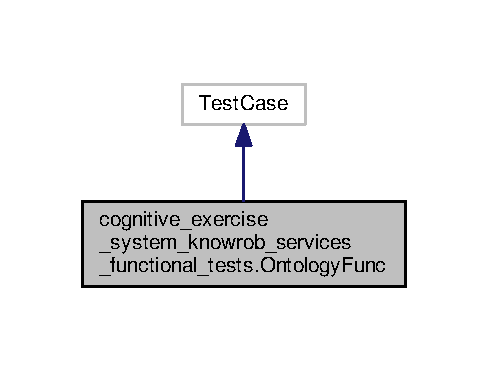
\includegraphics[width=234pt]{classcognitive__exercise__system__knowrob__services__functional__tests_1_1OntologyFunc__inherit__graph}
\end{center}
\end{figure}


Collaboration diagram for cognitive\-\_\-exercise\-\_\-system\-\_\-knowrob\-\_\-services\-\_\-functional\-\_\-tests.\-Ontology\-Func\-:
\nopagebreak
\begin{figure}[H]
\begin{center}
\leavevmode
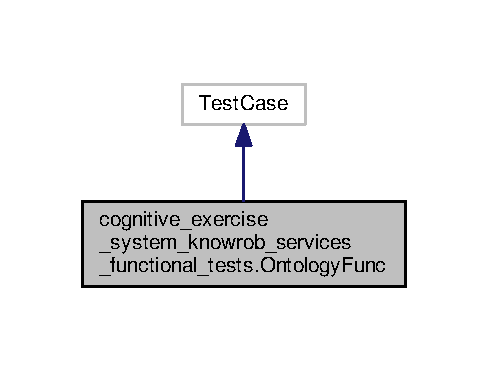
\includegraphics[width=234pt]{classcognitive__exercise__system__knowrob__services__functional__tests_1_1OntologyFunc__coll__graph}
\end{center}
\end{figure}
\subsection*{Public Member Functions}
\begin{DoxyCompactItemize}
\item 
def \hyperlink{classcognitive__exercise__system__knowrob__services__functional__tests_1_1OntologyFunc_a55d3ca0e805f218c0334a17e6a5ad73f}{test\-\_\-cognitive\-\_\-tests\-\_\-of\-\_\-existent\-\_\-type}
\begin{DoxyCompactList}\small\item\em Test cognitive tests of existent type. \end{DoxyCompactList}\item 
def \hyperlink{classcognitive__exercise__system__knowrob__services__functional__tests_1_1OntologyFunc_a651c94c6b07b35dd8b9b3a66045ac502}{test\-\_\-cognitive\-\_\-tests\-\_\-of\-\_\-nonexistent\-\_\-type}
\begin{DoxyCompactList}\small\item\em Test cognitive tests of non existent type. \end{DoxyCompactList}\item 
def \hyperlink{classcognitive__exercise__system__knowrob__services__functional__tests_1_1OntologyFunc_af4ed2d90b352171d1cd40a6bc09f951d}{test\-\_\-create\-\_\-nonexistent\-\_\-cognitive\-\_\-test}
\begin{DoxyCompactList}\small\item\em Test create existent cognitive test def test\-\_\-create\-\_\-existent\-\_\-cognitive\-\_\-test(self)\-: subclasses\-\_\-of\-\_\-service = rospy.\-get\-\_\-param(\textbackslash{} \char`\"{}rapp\-\_\-knowrob\-\_\-wrapper\-\_\-create\-\_\-cognitve\-\_\-tests\char`\"{}) rospy.\-wait\-\_\-for\-\_\-service(subclasses\-\_\-of\-\_\-service) \end{DoxyCompactList}\item 
def \hyperlink{classcognitive__exercise__system__knowrob__services__functional__tests_1_1OntologyFunc_a60ac919b56f4153fb3c7e5f7149eedb3}{test\-\_\-create\-\_\-nonexistent\-\_\-cognitive\-\_\-test\-\_\-xml\-\_\-path\-\_\-nonexistent}
\begin{DoxyCompactList}\small\item\em Test create non existent cognitive test with invalid xml path. \end{DoxyCompactList}\item 
def \hyperlink{classcognitive__exercise__system__knowrob__services__functional__tests_1_1OntologyFunc_a3c9113598b5d2f42d439a4965db22d9d}{test\-\_\-get\-\_\-user\-\_\-ontology\-\_\-alias\-\_\-existent\-\_\-user}
\begin{DoxyCompactList}\small\item\em Test get user ontology alias of existent user. \end{DoxyCompactList}\item 
def \hyperlink{classcognitive__exercise__system__knowrob__services__functional__tests_1_1OntologyFunc_af2dd09a1ea405c586906a8db0b4de689}{test\-\_\-get\-\_\-user\-\_\-ontology\-\_\-alias\-\_\-nonexistent\-\_\-user}
\begin{DoxyCompactList}\small\item\em Test get user ontology alias of nonexistent user. \end{DoxyCompactList}\item 
def \hyperlink{classcognitive__exercise__system__knowrob__services__functional__tests_1_1OntologyFunc_ab2bcb296c17b73a1baa76c55ffdade52}{test\-\_\-record\-\_\-user\-\_\-performance\-\_\-nonexisting\-\_\-test\-\_\-and\-\_\-user}
\begin{DoxyCompactList}\small\item\em Test record user performance of existent user and test type def test\-\_\-record\-\_\-user\-\_\-performance\-\_\-existing\-\_\-test\-\_\-and\-\_\-user(self)\-: subclasses\-\_\-of\-\_\-service = rospy.\-get\-\_\-param(\textbackslash{} \char`\"{}rapp\-\_\-knowrob\-\_\-wrapper\-\_\-record\-\_\-user\-\_\-cognitive\-\_\-tests\-\_\-performance\char`\"{}) rospy.\-wait\-\_\-for\-\_\-service(subclasses\-\_\-of\-\_\-service) \end{DoxyCompactList}\item 
def \hyperlink{classcognitive__exercise__system__knowrob__services__functional__tests_1_1OntologyFunc_a7589b1b87bf171a7b19fb1620e689c4b}{test\-\_\-user\-\_\-performance\-\_\-existent\-\_\-user\-\_\-and\-\_\-test}
\begin{DoxyCompactList}\small\item\em Test user performance of existent user and test type. \end{DoxyCompactList}\item 
def \hyperlink{classcognitive__exercise__system__knowrob__services__functional__tests_1_1OntologyFunc_ad697dd9b6de9014f73d1deda76e17abf}{test\-\_\-user\-\_\-performance\-\_\-nonexistent\-\_\-user\-\_\-and\-\_\-test}
\begin{DoxyCompactList}\small\item\em Test user performance of nonexistent user and test type. \end{DoxyCompactList}\end{DoxyCompactItemize}


\subsection{Detailed Description}
Inherits the unittest.\-Test\-Case class in order to offer functional tests functionality. 

Definition at line 44 of file cognitive\-\_\-exercise\-\_\-system\-\_\-knowrob\-\_\-services\-\_\-functional\-\_\-tests.\-py.



\subsection{Member Function Documentation}
\hypertarget{classcognitive__exercise__system__knowrob__services__functional__tests_1_1OntologyFunc_a55d3ca0e805f218c0334a17e6a5ad73f}{\index{cognitive\-\_\-exercise\-\_\-system\-\_\-knowrob\-\_\-services\-\_\-functional\-\_\-tests\-::\-Ontology\-Func@{cognitive\-\_\-exercise\-\_\-system\-\_\-knowrob\-\_\-services\-\_\-functional\-\_\-tests\-::\-Ontology\-Func}!test\-\_\-cognitive\-\_\-tests\-\_\-of\-\_\-existent\-\_\-type@{test\-\_\-cognitive\-\_\-tests\-\_\-of\-\_\-existent\-\_\-type}}
\index{test\-\_\-cognitive\-\_\-tests\-\_\-of\-\_\-existent\-\_\-type@{test\-\_\-cognitive\-\_\-tests\-\_\-of\-\_\-existent\-\_\-type}!cognitive_exercise_system_knowrob_services_functional_tests::OntologyFunc@{cognitive\-\_\-exercise\-\_\-system\-\_\-knowrob\-\_\-services\-\_\-functional\-\_\-tests\-::\-Ontology\-Func}}
\subsubsection[{test\-\_\-cognitive\-\_\-tests\-\_\-of\-\_\-existent\-\_\-type}]{\setlength{\rightskip}{0pt plus 5cm}def cognitive\-\_\-exercise\-\_\-system\-\_\-knowrob\-\_\-services\-\_\-functional\-\_\-tests.\-Ontology\-Func.\-test\-\_\-cognitive\-\_\-tests\-\_\-of\-\_\-existent\-\_\-type (
\begin{DoxyParamCaption}
\item[{}]{self}
\end{DoxyParamCaption}
)}}\label{classcognitive__exercise__system__knowrob__services__functional__tests_1_1OntologyFunc_a55d3ca0e805f218c0334a17e6a5ad73f}


Test cognitive tests of existent type. 



Definition at line 47 of file cognitive\-\_\-exercise\-\_\-system\-\_\-knowrob\-\_\-services\-\_\-functional\-\_\-tests.\-py.

\hypertarget{classcognitive__exercise__system__knowrob__services__functional__tests_1_1OntologyFunc_a651c94c6b07b35dd8b9b3a66045ac502}{\index{cognitive\-\_\-exercise\-\_\-system\-\_\-knowrob\-\_\-services\-\_\-functional\-\_\-tests\-::\-Ontology\-Func@{cognitive\-\_\-exercise\-\_\-system\-\_\-knowrob\-\_\-services\-\_\-functional\-\_\-tests\-::\-Ontology\-Func}!test\-\_\-cognitive\-\_\-tests\-\_\-of\-\_\-nonexistent\-\_\-type@{test\-\_\-cognitive\-\_\-tests\-\_\-of\-\_\-nonexistent\-\_\-type}}
\index{test\-\_\-cognitive\-\_\-tests\-\_\-of\-\_\-nonexistent\-\_\-type@{test\-\_\-cognitive\-\_\-tests\-\_\-of\-\_\-nonexistent\-\_\-type}!cognitive_exercise_system_knowrob_services_functional_tests::OntologyFunc@{cognitive\-\_\-exercise\-\_\-system\-\_\-knowrob\-\_\-services\-\_\-functional\-\_\-tests\-::\-Ontology\-Func}}
\subsubsection[{test\-\_\-cognitive\-\_\-tests\-\_\-of\-\_\-nonexistent\-\_\-type}]{\setlength{\rightskip}{0pt plus 5cm}def cognitive\-\_\-exercise\-\_\-system\-\_\-knowrob\-\_\-services\-\_\-functional\-\_\-tests.\-Ontology\-Func.\-test\-\_\-cognitive\-\_\-tests\-\_\-of\-\_\-nonexistent\-\_\-type (
\begin{DoxyParamCaption}
\item[{}]{self}
\end{DoxyParamCaption}
)}}\label{classcognitive__exercise__system__knowrob__services__functional__tests_1_1OntologyFunc_a651c94c6b07b35dd8b9b3a66045ac502}


Test cognitive tests of non existent type. 



Definition at line 65 of file cognitive\-\_\-exercise\-\_\-system\-\_\-knowrob\-\_\-services\-\_\-functional\-\_\-tests.\-py.

\hypertarget{classcognitive__exercise__system__knowrob__services__functional__tests_1_1OntologyFunc_af4ed2d90b352171d1cd40a6bc09f951d}{\index{cognitive\-\_\-exercise\-\_\-system\-\_\-knowrob\-\_\-services\-\_\-functional\-\_\-tests\-::\-Ontology\-Func@{cognitive\-\_\-exercise\-\_\-system\-\_\-knowrob\-\_\-services\-\_\-functional\-\_\-tests\-::\-Ontology\-Func}!test\-\_\-create\-\_\-nonexistent\-\_\-cognitive\-\_\-test@{test\-\_\-create\-\_\-nonexistent\-\_\-cognitive\-\_\-test}}
\index{test\-\_\-create\-\_\-nonexistent\-\_\-cognitive\-\_\-test@{test\-\_\-create\-\_\-nonexistent\-\_\-cognitive\-\_\-test}!cognitive_exercise_system_knowrob_services_functional_tests::OntologyFunc@{cognitive\-\_\-exercise\-\_\-system\-\_\-knowrob\-\_\-services\-\_\-functional\-\_\-tests\-::\-Ontology\-Func}}
\subsubsection[{test\-\_\-create\-\_\-nonexistent\-\_\-cognitive\-\_\-test}]{\setlength{\rightskip}{0pt plus 5cm}def cognitive\-\_\-exercise\-\_\-system\-\_\-knowrob\-\_\-services\-\_\-functional\-\_\-tests.\-Ontology\-Func.\-test\-\_\-create\-\_\-nonexistent\-\_\-cognitive\-\_\-test (
\begin{DoxyParamCaption}
\item[{}]{self}
\end{DoxyParamCaption}
)}}\label{classcognitive__exercise__system__knowrob__services__functional__tests_1_1OntologyFunc_af4ed2d90b352171d1cd40a6bc09f951d}


Test create existent cognitive test def test\-\_\-create\-\_\-existent\-\_\-cognitive\-\_\-test(self)\-: subclasses\-\_\-of\-\_\-service = rospy.\-get\-\_\-param(\textbackslash{} \char`\"{}rapp\-\_\-knowrob\-\_\-wrapper\-\_\-create\-\_\-cognitve\-\_\-tests\char`\"{}) rospy.\-wait\-\_\-for\-\_\-service(subclasses\-\_\-of\-\_\-service) 

Test create non existent cognitive test 

Definition at line 196 of file cognitive\-\_\-exercise\-\_\-system\-\_\-knowrob\-\_\-services\-\_\-functional\-\_\-tests.\-py.

\hypertarget{classcognitive__exercise__system__knowrob__services__functional__tests_1_1OntologyFunc_a60ac919b56f4153fb3c7e5f7149eedb3}{\index{cognitive\-\_\-exercise\-\_\-system\-\_\-knowrob\-\_\-services\-\_\-functional\-\_\-tests\-::\-Ontology\-Func@{cognitive\-\_\-exercise\-\_\-system\-\_\-knowrob\-\_\-services\-\_\-functional\-\_\-tests\-::\-Ontology\-Func}!test\-\_\-create\-\_\-nonexistent\-\_\-cognitive\-\_\-test\-\_\-xml\-\_\-path\-\_\-nonexistent@{test\-\_\-create\-\_\-nonexistent\-\_\-cognitive\-\_\-test\-\_\-xml\-\_\-path\-\_\-nonexistent}}
\index{test\-\_\-create\-\_\-nonexistent\-\_\-cognitive\-\_\-test\-\_\-xml\-\_\-path\-\_\-nonexistent@{test\-\_\-create\-\_\-nonexistent\-\_\-cognitive\-\_\-test\-\_\-xml\-\_\-path\-\_\-nonexistent}!cognitive_exercise_system_knowrob_services_functional_tests::OntologyFunc@{cognitive\-\_\-exercise\-\_\-system\-\_\-knowrob\-\_\-services\-\_\-functional\-\_\-tests\-::\-Ontology\-Func}}
\subsubsection[{test\-\_\-create\-\_\-nonexistent\-\_\-cognitive\-\_\-test\-\_\-xml\-\_\-path\-\_\-nonexistent}]{\setlength{\rightskip}{0pt plus 5cm}def cognitive\-\_\-exercise\-\_\-system\-\_\-knowrob\-\_\-services\-\_\-functional\-\_\-tests.\-Ontology\-Func.\-test\-\_\-create\-\_\-nonexistent\-\_\-cognitive\-\_\-test\-\_\-xml\-\_\-path\-\_\-nonexistent (
\begin{DoxyParamCaption}
\item[{}]{self}
\end{DoxyParamCaption}
)}}\label{classcognitive__exercise__system__knowrob__services__functional__tests_1_1OntologyFunc_a60ac919b56f4153fb3c7e5f7149eedb3}


Test create non existent cognitive test with invalid xml path. 



Definition at line 216 of file cognitive\-\_\-exercise\-\_\-system\-\_\-knowrob\-\_\-services\-\_\-functional\-\_\-tests.\-py.

\hypertarget{classcognitive__exercise__system__knowrob__services__functional__tests_1_1OntologyFunc_a3c9113598b5d2f42d439a4965db22d9d}{\index{cognitive\-\_\-exercise\-\_\-system\-\_\-knowrob\-\_\-services\-\_\-functional\-\_\-tests\-::\-Ontology\-Func@{cognitive\-\_\-exercise\-\_\-system\-\_\-knowrob\-\_\-services\-\_\-functional\-\_\-tests\-::\-Ontology\-Func}!test\-\_\-get\-\_\-user\-\_\-ontology\-\_\-alias\-\_\-existent\-\_\-user@{test\-\_\-get\-\_\-user\-\_\-ontology\-\_\-alias\-\_\-existent\-\_\-user}}
\index{test\-\_\-get\-\_\-user\-\_\-ontology\-\_\-alias\-\_\-existent\-\_\-user@{test\-\_\-get\-\_\-user\-\_\-ontology\-\_\-alias\-\_\-existent\-\_\-user}!cognitive_exercise_system_knowrob_services_functional_tests::OntologyFunc@{cognitive\-\_\-exercise\-\_\-system\-\_\-knowrob\-\_\-services\-\_\-functional\-\_\-tests\-::\-Ontology\-Func}}
\subsubsection[{test\-\_\-get\-\_\-user\-\_\-ontology\-\_\-alias\-\_\-existent\-\_\-user}]{\setlength{\rightskip}{0pt plus 5cm}def cognitive\-\_\-exercise\-\_\-system\-\_\-knowrob\-\_\-services\-\_\-functional\-\_\-tests.\-Ontology\-Func.\-test\-\_\-get\-\_\-user\-\_\-ontology\-\_\-alias\-\_\-existent\-\_\-user (
\begin{DoxyParamCaption}
\item[{}]{self}
\end{DoxyParamCaption}
)}}\label{classcognitive__exercise__system__knowrob__services__functional__tests_1_1OntologyFunc_a3c9113598b5d2f42d439a4965db22d9d}


Test get user ontology alias of existent user. 



Definition at line 81 of file cognitive\-\_\-exercise\-\_\-system\-\_\-knowrob\-\_\-services\-\_\-functional\-\_\-tests.\-py.

\hypertarget{classcognitive__exercise__system__knowrob__services__functional__tests_1_1OntologyFunc_af2dd09a1ea405c586906a8db0b4de689}{\index{cognitive\-\_\-exercise\-\_\-system\-\_\-knowrob\-\_\-services\-\_\-functional\-\_\-tests\-::\-Ontology\-Func@{cognitive\-\_\-exercise\-\_\-system\-\_\-knowrob\-\_\-services\-\_\-functional\-\_\-tests\-::\-Ontology\-Func}!test\-\_\-get\-\_\-user\-\_\-ontology\-\_\-alias\-\_\-nonexistent\-\_\-user@{test\-\_\-get\-\_\-user\-\_\-ontology\-\_\-alias\-\_\-nonexistent\-\_\-user}}
\index{test\-\_\-get\-\_\-user\-\_\-ontology\-\_\-alias\-\_\-nonexistent\-\_\-user@{test\-\_\-get\-\_\-user\-\_\-ontology\-\_\-alias\-\_\-nonexistent\-\_\-user}!cognitive_exercise_system_knowrob_services_functional_tests::OntologyFunc@{cognitive\-\_\-exercise\-\_\-system\-\_\-knowrob\-\_\-services\-\_\-functional\-\_\-tests\-::\-Ontology\-Func}}
\subsubsection[{test\-\_\-get\-\_\-user\-\_\-ontology\-\_\-alias\-\_\-nonexistent\-\_\-user}]{\setlength{\rightskip}{0pt plus 5cm}def cognitive\-\_\-exercise\-\_\-system\-\_\-knowrob\-\_\-services\-\_\-functional\-\_\-tests.\-Ontology\-Func.\-test\-\_\-get\-\_\-user\-\_\-ontology\-\_\-alias\-\_\-nonexistent\-\_\-user (
\begin{DoxyParamCaption}
\item[{}]{self}
\end{DoxyParamCaption}
)}}\label{classcognitive__exercise__system__knowrob__services__functional__tests_1_1OntologyFunc_af2dd09a1ea405c586906a8db0b4de689}


Test get user ontology alias of nonexistent user. 



Definition at line 96 of file cognitive\-\_\-exercise\-\_\-system\-\_\-knowrob\-\_\-services\-\_\-functional\-\_\-tests.\-py.

\hypertarget{classcognitive__exercise__system__knowrob__services__functional__tests_1_1OntologyFunc_ab2bcb296c17b73a1baa76c55ffdade52}{\index{cognitive\-\_\-exercise\-\_\-system\-\_\-knowrob\-\_\-services\-\_\-functional\-\_\-tests\-::\-Ontology\-Func@{cognitive\-\_\-exercise\-\_\-system\-\_\-knowrob\-\_\-services\-\_\-functional\-\_\-tests\-::\-Ontology\-Func}!test\-\_\-record\-\_\-user\-\_\-performance\-\_\-nonexisting\-\_\-test\-\_\-and\-\_\-user@{test\-\_\-record\-\_\-user\-\_\-performance\-\_\-nonexisting\-\_\-test\-\_\-and\-\_\-user}}
\index{test\-\_\-record\-\_\-user\-\_\-performance\-\_\-nonexisting\-\_\-test\-\_\-and\-\_\-user@{test\-\_\-record\-\_\-user\-\_\-performance\-\_\-nonexisting\-\_\-test\-\_\-and\-\_\-user}!cognitive_exercise_system_knowrob_services_functional_tests::OntologyFunc@{cognitive\-\_\-exercise\-\_\-system\-\_\-knowrob\-\_\-services\-\_\-functional\-\_\-tests\-::\-Ontology\-Func}}
\subsubsection[{test\-\_\-record\-\_\-user\-\_\-performance\-\_\-nonexisting\-\_\-test\-\_\-and\-\_\-user}]{\setlength{\rightskip}{0pt plus 5cm}def cognitive\-\_\-exercise\-\_\-system\-\_\-knowrob\-\_\-services\-\_\-functional\-\_\-tests.\-Ontology\-Func.\-test\-\_\-record\-\_\-user\-\_\-performance\-\_\-nonexisting\-\_\-test\-\_\-and\-\_\-user (
\begin{DoxyParamCaption}
\item[{}]{self}
\end{DoxyParamCaption}
)}}\label{classcognitive__exercise__system__knowrob__services__functional__tests_1_1OntologyFunc_ab2bcb296c17b73a1baa76c55ffdade52}


Test record user performance of existent user and test type def test\-\_\-record\-\_\-user\-\_\-performance\-\_\-existing\-\_\-test\-\_\-and\-\_\-user(self)\-: subclasses\-\_\-of\-\_\-service = rospy.\-get\-\_\-param(\textbackslash{} \char`\"{}rapp\-\_\-knowrob\-\_\-wrapper\-\_\-record\-\_\-user\-\_\-cognitive\-\_\-tests\-\_\-performance\char`\"{}) rospy.\-wait\-\_\-for\-\_\-service(subclasses\-\_\-of\-\_\-service) 

req.\-test\-\_\-type=\char`\"{}\-Arithmetic\-Cts\char`\"{} req.\-test=\char`\"{}\-Arithmetic\-Cts\-\_\-\-Mewmm\-Es\-P\char`\"{} req.\-score=11 req.\-timestamp=1 response = test\-\_\-service(req) self.\-assert\-Equal(response.\-success, True) Test record user performance of nonexistent user and test type 

Definition at line 161 of file cognitive\-\_\-exercise\-\_\-system\-\_\-knowrob\-\_\-services\-\_\-functional\-\_\-tests.\-py.

\hypertarget{classcognitive__exercise__system__knowrob__services__functional__tests_1_1OntologyFunc_a7589b1b87bf171a7b19fb1620e689c4b}{\index{cognitive\-\_\-exercise\-\_\-system\-\_\-knowrob\-\_\-services\-\_\-functional\-\_\-tests\-::\-Ontology\-Func@{cognitive\-\_\-exercise\-\_\-system\-\_\-knowrob\-\_\-services\-\_\-functional\-\_\-tests\-::\-Ontology\-Func}!test\-\_\-user\-\_\-performance\-\_\-existent\-\_\-user\-\_\-and\-\_\-test@{test\-\_\-user\-\_\-performance\-\_\-existent\-\_\-user\-\_\-and\-\_\-test}}
\index{test\-\_\-user\-\_\-performance\-\_\-existent\-\_\-user\-\_\-and\-\_\-test@{test\-\_\-user\-\_\-performance\-\_\-existent\-\_\-user\-\_\-and\-\_\-test}!cognitive_exercise_system_knowrob_services_functional_tests::OntologyFunc@{cognitive\-\_\-exercise\-\_\-system\-\_\-knowrob\-\_\-services\-\_\-functional\-\_\-tests\-::\-Ontology\-Func}}
\subsubsection[{test\-\_\-user\-\_\-performance\-\_\-existent\-\_\-user\-\_\-and\-\_\-test}]{\setlength{\rightskip}{0pt plus 5cm}def cognitive\-\_\-exercise\-\_\-system\-\_\-knowrob\-\_\-services\-\_\-functional\-\_\-tests.\-Ontology\-Func.\-test\-\_\-user\-\_\-performance\-\_\-existent\-\_\-user\-\_\-and\-\_\-test (
\begin{DoxyParamCaption}
\item[{}]{self}
\end{DoxyParamCaption}
)}}\label{classcognitive__exercise__system__knowrob__services__functional__tests_1_1OntologyFunc_a7589b1b87bf171a7b19fb1620e689c4b}


Test user performance of existent user and test type. 



Definition at line 110 of file cognitive\-\_\-exercise\-\_\-system\-\_\-knowrob\-\_\-services\-\_\-functional\-\_\-tests.\-py.

\hypertarget{classcognitive__exercise__system__knowrob__services__functional__tests_1_1OntologyFunc_ad697dd9b6de9014f73d1deda76e17abf}{\index{cognitive\-\_\-exercise\-\_\-system\-\_\-knowrob\-\_\-services\-\_\-functional\-\_\-tests\-::\-Ontology\-Func@{cognitive\-\_\-exercise\-\_\-system\-\_\-knowrob\-\_\-services\-\_\-functional\-\_\-tests\-::\-Ontology\-Func}!test\-\_\-user\-\_\-performance\-\_\-nonexistent\-\_\-user\-\_\-and\-\_\-test@{test\-\_\-user\-\_\-performance\-\_\-nonexistent\-\_\-user\-\_\-and\-\_\-test}}
\index{test\-\_\-user\-\_\-performance\-\_\-nonexistent\-\_\-user\-\_\-and\-\_\-test@{test\-\_\-user\-\_\-performance\-\_\-nonexistent\-\_\-user\-\_\-and\-\_\-test}!cognitive_exercise_system_knowrob_services_functional_tests::OntologyFunc@{cognitive\-\_\-exercise\-\_\-system\-\_\-knowrob\-\_\-services\-\_\-functional\-\_\-tests\-::\-Ontology\-Func}}
\subsubsection[{test\-\_\-user\-\_\-performance\-\_\-nonexistent\-\_\-user\-\_\-and\-\_\-test}]{\setlength{\rightskip}{0pt plus 5cm}def cognitive\-\_\-exercise\-\_\-system\-\_\-knowrob\-\_\-services\-\_\-functional\-\_\-tests.\-Ontology\-Func.\-test\-\_\-user\-\_\-performance\-\_\-nonexistent\-\_\-user\-\_\-and\-\_\-test (
\begin{DoxyParamCaption}
\item[{}]{self}
\end{DoxyParamCaption}
)}}\label{classcognitive__exercise__system__knowrob__services__functional__tests_1_1OntologyFunc_ad697dd9b6de9014f73d1deda76e17abf}


Test user performance of nonexistent user and test type. 



Definition at line 127 of file cognitive\-\_\-exercise\-\_\-system\-\_\-knowrob\-\_\-services\-\_\-functional\-\_\-tests.\-py.



The documentation for this class was generated from the following file\-:\begin{DoxyCompactItemize}
\item 
/home/travis/rapp\-\_\-temp/rapp-\/platform/rapp\-\_\-knowrob\-\_\-wrapper/tests/functional/\hyperlink{cognitive__exercise__system__knowrob__services__functional__tests_8py}{cognitive\-\_\-exercise\-\_\-system\-\_\-knowrob\-\_\-services\-\_\-functional\-\_\-tests.\-py}\end{DoxyCompactItemize}

\hypertarget{classload__dump__ontology__functional__tests_1_1OntologyFunc}{\section{load\-\_\-dump\-\_\-ontology\-\_\-functional\-\_\-tests.\-Ontology\-Func Class Reference}
\label{classload__dump__ontology__functional__tests_1_1OntologyFunc}\index{load\-\_\-dump\-\_\-ontology\-\_\-functional\-\_\-tests.\-Ontology\-Func@{load\-\_\-dump\-\_\-ontology\-\_\-functional\-\_\-tests.\-Ontology\-Func}}
}


Inherits the unittest.\-Test\-Case class in order to offer functional tests functionalit.  




Inheritance diagram for load\-\_\-dump\-\_\-ontology\-\_\-functional\-\_\-tests.\-Ontology\-Func\-:


Collaboration diagram for load\-\_\-dump\-\_\-ontology\-\_\-functional\-\_\-tests.\-Ontology\-Func\-:
\subsection*{Public Member Functions}
\begin{DoxyCompactItemize}
\item 
def \hyperlink{classload__dump__ontology__functional__tests_1_1OntologyFunc_ad50d52bac563582e9052c61a9a9d5196}{test\-\_\-dump\-\_\-correct\-\_\-path}
\begin{DoxyCompactList}\small\item\em Test dump ontology with correct path. \end{DoxyCompactList}\item 
def \hyperlink{classload__dump__ontology__functional__tests_1_1OntologyFunc_a208ccc161865a0fc32bfc3c1af7d27a0}{test\-\_\-dump\-\_\-invalid\-\_\-path}
\begin{DoxyCompactList}\small\item\em Test dump ontology with invalid path. \end{DoxyCompactList}\item 
def \hyperlink{classload__dump__ontology__functional__tests_1_1OntologyFunc_a598f0f8220f6d038667c0ab4f29ed851}{test\-\_\-load\-\_\-existent}
\begin{DoxyCompactList}\small\item\em Test load ontology from existent file. \end{DoxyCompactList}\item 
def \hyperlink{classload__dump__ontology__functional__tests_1_1OntologyFunc_a8642dbfe9f5b4b7ebd0a4ab5b52c605c}{test\-\_\-load\-\_\-nonexistent}
\begin{DoxyCompactList}\small\item\em Test load ontology from non existent file. \end{DoxyCompactList}\end{DoxyCompactItemize}


\subsection{Detailed Description}
Inherits the unittest.\-Test\-Case class in order to offer functional tests functionalit. 

Definition at line 33 of file load\-\_\-dump\-\_\-ontology\-\_\-functional\-\_\-tests.\-py.



\subsection{Member Function Documentation}
\hypertarget{classload__dump__ontology__functional__tests_1_1OntologyFunc_ad50d52bac563582e9052c61a9a9d5196}{\index{load\-\_\-dump\-\_\-ontology\-\_\-functional\-\_\-tests\-::\-Ontology\-Func@{load\-\_\-dump\-\_\-ontology\-\_\-functional\-\_\-tests\-::\-Ontology\-Func}!test\-\_\-dump\-\_\-correct\-\_\-path@{test\-\_\-dump\-\_\-correct\-\_\-path}}
\index{test\-\_\-dump\-\_\-correct\-\_\-path@{test\-\_\-dump\-\_\-correct\-\_\-path}!load_dump_ontology_functional_tests::OntologyFunc@{load\-\_\-dump\-\_\-ontology\-\_\-functional\-\_\-tests\-::\-Ontology\-Func}}
\subsubsection[{test\-\_\-dump\-\_\-correct\-\_\-path}]{\setlength{\rightskip}{0pt plus 5cm}def load\-\_\-dump\-\_\-ontology\-\_\-functional\-\_\-tests.\-Ontology\-Func.\-test\-\_\-dump\-\_\-correct\-\_\-path (
\begin{DoxyParamCaption}
\item[{}]{self}
\end{DoxyParamCaption}
)}}\label{classload__dump__ontology__functional__tests_1_1OntologyFunc_ad50d52bac563582e9052c61a9a9d5196}


Test dump ontology with correct path. 



Definition at line 64 of file load\-\_\-dump\-\_\-ontology\-\_\-functional\-\_\-tests.\-py.

\hypertarget{classload__dump__ontology__functional__tests_1_1OntologyFunc_a208ccc161865a0fc32bfc3c1af7d27a0}{\index{load\-\_\-dump\-\_\-ontology\-\_\-functional\-\_\-tests\-::\-Ontology\-Func@{load\-\_\-dump\-\_\-ontology\-\_\-functional\-\_\-tests\-::\-Ontology\-Func}!test\-\_\-dump\-\_\-invalid\-\_\-path@{test\-\_\-dump\-\_\-invalid\-\_\-path}}
\index{test\-\_\-dump\-\_\-invalid\-\_\-path@{test\-\_\-dump\-\_\-invalid\-\_\-path}!load_dump_ontology_functional_tests::OntologyFunc@{load\-\_\-dump\-\_\-ontology\-\_\-functional\-\_\-tests\-::\-Ontology\-Func}}
\subsubsection[{test\-\_\-dump\-\_\-invalid\-\_\-path}]{\setlength{\rightskip}{0pt plus 5cm}def load\-\_\-dump\-\_\-ontology\-\_\-functional\-\_\-tests.\-Ontology\-Func.\-test\-\_\-dump\-\_\-invalid\-\_\-path (
\begin{DoxyParamCaption}
\item[{}]{self}
\end{DoxyParamCaption}
)}}\label{classload__dump__ontology__functional__tests_1_1OntologyFunc_a208ccc161865a0fc32bfc3c1af7d27a0}


Test dump ontology with invalid path. 



Definition at line 78 of file load\-\_\-dump\-\_\-ontology\-\_\-functional\-\_\-tests.\-py.

\hypertarget{classload__dump__ontology__functional__tests_1_1OntologyFunc_a598f0f8220f6d038667c0ab4f29ed851}{\index{load\-\_\-dump\-\_\-ontology\-\_\-functional\-\_\-tests\-::\-Ontology\-Func@{load\-\_\-dump\-\_\-ontology\-\_\-functional\-\_\-tests\-::\-Ontology\-Func}!test\-\_\-load\-\_\-existent@{test\-\_\-load\-\_\-existent}}
\index{test\-\_\-load\-\_\-existent@{test\-\_\-load\-\_\-existent}!load_dump_ontology_functional_tests::OntologyFunc@{load\-\_\-dump\-\_\-ontology\-\_\-functional\-\_\-tests\-::\-Ontology\-Func}}
\subsubsection[{test\-\_\-load\-\_\-existent}]{\setlength{\rightskip}{0pt plus 5cm}def load\-\_\-dump\-\_\-ontology\-\_\-functional\-\_\-tests.\-Ontology\-Func.\-test\-\_\-load\-\_\-existent (
\begin{DoxyParamCaption}
\item[{}]{self}
\end{DoxyParamCaption}
)}}\label{classload__dump__ontology__functional__tests_1_1OntologyFunc_a598f0f8220f6d038667c0ab4f29ed851}


Test load ontology from existent file. 



Definition at line 36 of file load\-\_\-dump\-\_\-ontology\-\_\-functional\-\_\-tests.\-py.

\hypertarget{classload__dump__ontology__functional__tests_1_1OntologyFunc_a8642dbfe9f5b4b7ebd0a4ab5b52c605c}{\index{load\-\_\-dump\-\_\-ontology\-\_\-functional\-\_\-tests\-::\-Ontology\-Func@{load\-\_\-dump\-\_\-ontology\-\_\-functional\-\_\-tests\-::\-Ontology\-Func}!test\-\_\-load\-\_\-nonexistent@{test\-\_\-load\-\_\-nonexistent}}
\index{test\-\_\-load\-\_\-nonexistent@{test\-\_\-load\-\_\-nonexistent}!load_dump_ontology_functional_tests::OntologyFunc@{load\-\_\-dump\-\_\-ontology\-\_\-functional\-\_\-tests\-::\-Ontology\-Func}}
\subsubsection[{test\-\_\-load\-\_\-nonexistent}]{\setlength{\rightskip}{0pt plus 5cm}def load\-\_\-dump\-\_\-ontology\-\_\-functional\-\_\-tests.\-Ontology\-Func.\-test\-\_\-load\-\_\-nonexistent (
\begin{DoxyParamCaption}
\item[{}]{self}
\end{DoxyParamCaption}
)}}\label{classload__dump__ontology__functional__tests_1_1OntologyFunc_a8642dbfe9f5b4b7ebd0a4ab5b52c605c}


Test load ontology from non existent file. 



Definition at line 50 of file load\-\_\-dump\-\_\-ontology\-\_\-functional\-\_\-tests.\-py.



The documentation for this class was generated from the following file\-:\begin{DoxyCompactItemize}
\item 
/home/travis/rapp\-\_\-temp/rapp-\/platform/rapp\-\_\-knowrob\-\_\-wrapper/tests/functional/\hyperlink{load__dump__ontology__functional__tests_8py}{load\-\_\-dump\-\_\-ontology\-\_\-functional\-\_\-tests.\-py}\end{DoxyCompactItemize}

\hypertarget{classsub__super__class__functional__tests_1_1OntologyFunc}{\section{sub\-\_\-super\-\_\-class\-\_\-functional\-\_\-tests.\-Ontology\-Func Class Reference}
\label{classsub__super__class__functional__tests_1_1OntologyFunc}\index{sub\-\_\-super\-\_\-class\-\_\-functional\-\_\-tests.\-Ontology\-Func@{sub\-\_\-super\-\_\-class\-\_\-functional\-\_\-tests.\-Ontology\-Func}}
}


Inherits the unittest.\-Test\-Case class in order to offer functional tests functionality.  




Inheritance diagram for sub\-\_\-super\-\_\-class\-\_\-functional\-\_\-tests.\-Ontology\-Func\-:
\nopagebreak
\begin{figure}[H]
\begin{center}
\leavevmode
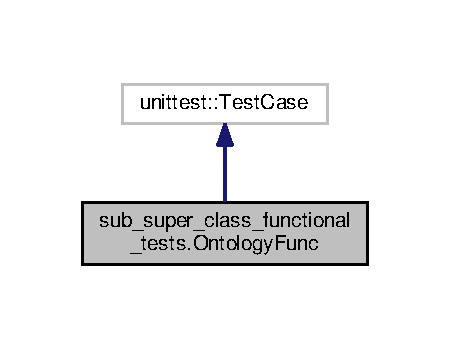
\includegraphics[width=216pt]{classsub__super__class__functional__tests_1_1OntologyFunc__inherit__graph}
\end{center}
\end{figure}


Collaboration diagram for sub\-\_\-super\-\_\-class\-\_\-functional\-\_\-tests.\-Ontology\-Func\-:
\nopagebreak
\begin{figure}[H]
\begin{center}
\leavevmode
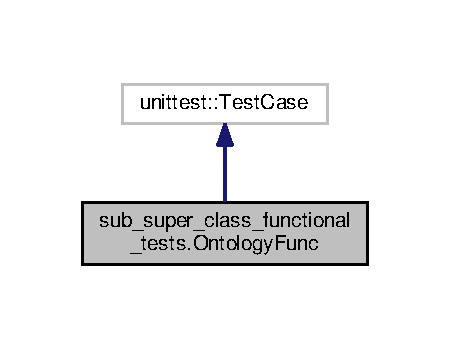
\includegraphics[width=216pt]{classsub__super__class__functional__tests_1_1OntologyFunc__coll__graph}
\end{center}
\end{figure}
\subsection*{Public Member Functions}
\begin{DoxyCompactItemize}
\item 
def \hyperlink{classsub__super__class__functional__tests_1_1OntologyFunc_a2c2269abc7334310c2033b85578563e3}{test\-\_\-sub\-\_\-superclasses\-\_\-of\-\_\-existent\-\_\-class\-\_\-direct}
\begin{DoxyCompactList}\small\item\em Tests sub-\/superclasses\-\_\-of existent class direct. \end{DoxyCompactList}\item 
def \hyperlink{classsub__super__class__functional__tests_1_1OntologyFunc_a9a68fde90b065a7ba950ff5566bbbcef}{test\-\_\-sub\-\_\-superclasses\-\_\-of\-\_\-existent\-\_\-class\-\_\-direct\-\_\-recursive}
\begin{DoxyCompactList}\small\item\em Tests sub-\/superclasses\-\_\-of existent class direct recursive. \end{DoxyCompactList}\item 
def \hyperlink{classsub__super__class__functional__tests_1_1OntologyFunc_a243cbc54adbf86cd3930aed9f4806dd4}{test\-\_\-sub\-\_\-superclasses\-\_\-of\-\_\-existent\-\_\-class\-\_\-indirect}
\begin{DoxyCompactList}\small\item\em Tests sub-\/superclasses\-\_\-of existent class indirect. \end{DoxyCompactList}\item 
def \hyperlink{classsub__super__class__functional__tests_1_1OntologyFunc_af62808d35d297753738a0d52ac0ffeb8}{test\-\_\-sub\-\_\-superclasses\-\_\-of\-\_\-existent\-\_\-class\-\_\-indirect\-\_\-recursive}
\begin{DoxyCompactList}\small\item\em Tests sub-\/superclasses\-\_\-of existent class indirect recursive. \end{DoxyCompactList}\item 
def \hyperlink{classsub__super__class__functional__tests_1_1OntologyFunc_a7e51e371afc2b76de676b15413659e18}{test\-\_\-sub\-\_\-superclasses\-\_\-of\-\_\-existent\-\_\-class\-\_\-recursive}
\begin{DoxyCompactList}\small\item\em Tests sub-\/superclasses\-\_\-of existent class recursive. \end{DoxyCompactList}\item 
def \hyperlink{classsub__super__class__functional__tests_1_1OntologyFunc_af184e6197eda380b2a70b99a2c7c2ede}{test\-\_\-sub\-\_\-superclasses\-\_\-of\-\_\-existent\-\_\-classes\-\_\-recursive}
\begin{DoxyCompactList}\small\item\em Tests sub-\/superclasses\-\_\-of existent classes. \end{DoxyCompactList}\item 
def \hyperlink{classsub__super__class__functional__tests_1_1OntologyFunc_adcc95b36fa9ee18896222f0bba6a7ec5}{test\-\_\-sub\-\_\-superclasses\-\_\-of\-\_\-non\-\_\-existent\-\_\-class}
\begin{DoxyCompactList}\small\item\em Tests sub-\/superclasses\-\_\-of non existent class. \end{DoxyCompactList}\item 
def \hyperlink{classsub__super__class__functional__tests_1_1OntologyFunc_ab7d45b5ec943915948005acc7d18facb}{test\-\_\-sub\-\_\-superclasses\-\_\-of\-\_\-non\-\_\-existent\-\_\-classes}
\begin{DoxyCompactList}\small\item\em Tests sub-\/superclasses\-\_\-of non existent classes. \end{DoxyCompactList}\item 
def \hyperlink{classsub__super__class__functional__tests_1_1OntologyFunc_ad293d2fb4c06fedde01c399221e8ee7d}{test\-\_\-subclasses\-\_\-of\-\_\-existent\-\_\-class}
\begin{DoxyCompactList}\small\item\em Tests Subclasses\-\_\-of existent class. \end{DoxyCompactList}\item 
def \hyperlink{classsub__super__class__functional__tests_1_1OntologyFunc_a992839ead105129dfb2cf2a4c95e7ef4}{test\-\_\-subclasses\-\_\-of\-\_\-existent\-\_\-class\-\_\-recursive}
\begin{DoxyCompactList}\small\item\em Tests Subclass\-\_\-of existent class recursive. \end{DoxyCompactList}\item 
def \hyperlink{classsub__super__class__functional__tests_1_1OntologyFunc_a972076ae8d5ad63906f97278e4eb0f8f}{test\-\_\-subclasses\-\_\-of\-\_\-existent\-\_\-class\-\_\-stress}
\begin{DoxyCompactList}\small\item\em Tests Subclasses\-\_\-of existent class stress. \end{DoxyCompactList}\item 
def \hyperlink{classsub__super__class__functional__tests_1_1OntologyFunc_a6768c2b4e4e8719a7db60df239af79c0}{test\-\_\-subclasses\-\_\-of\-\_\-non\-\_\-existent\-\_\-class}
\begin{DoxyCompactList}\small\item\em Tests Subclass\-\_\-of non existent class. \end{DoxyCompactList}\item 
def \hyperlink{classsub__super__class__functional__tests_1_1OntologyFunc_a93c10dafecd28a1a4ff9eec8c378e077}{test\-\_\-subclasses\-\_\-of\-\_\-non\-\_\-existent\-\_\-class\-\_\-recursive}
\begin{DoxyCompactList}\small\item\em Tests Subclass\-\_\-of non existent class recursive. \end{DoxyCompactList}\item 
def \hyperlink{classsub__super__class__functional__tests_1_1OntologyFunc_a7360ce5fe52a6f35f2c0a898d107d4d0}{test\-\_\-superclasses\-\_\-of\-\_\-existent\-\_\-class}
\begin{DoxyCompactList}\small\item\em Tests Superclasses\-\_\-of existent class. \end{DoxyCompactList}\item 
def \hyperlink{classsub__super__class__functional__tests_1_1OntologyFunc_a025f65f6a489c34f3875e6d2ab2a88fe}{test\-\_\-superclasses\-\_\-of\-\_\-existent\-\_\-class\-\_\-recursive}
\begin{DoxyCompactList}\small\item\em Tests Superclasses\-\_\-of existent class recursive. \end{DoxyCompactList}\item 
def \hyperlink{classsub__super__class__functional__tests_1_1OntologyFunc_a09984a286cd36ff5b6837874d8647c76}{test\-\_\-superclasses\-\_\-of\-\_\-non\-\_\-existent\-\_\-class}
\begin{DoxyCompactList}\small\item\em Tests Superclasses\-\_\-of non existent class. \end{DoxyCompactList}\item 
def \hyperlink{classsub__super__class__functional__tests_1_1OntologyFunc_a9865ddee876956c29db019d48cd94530}{test\-\_\-superclasses\-\_\-of\-\_\-non\-\_\-existent\-\_\-class\-\_\-recursive}
\begin{DoxyCompactList}\small\item\em Tests Superclasses\-\_\-of non existent class recursive. \end{DoxyCompactList}\end{DoxyCompactItemize}


\subsection{Detailed Description}
Inherits the unittest.\-Test\-Case class in order to offer functional tests functionality. 

Definition at line 38 of file sub\-\_\-super\-\_\-class\-\_\-functional\-\_\-tests.\-py.



\subsection{Member Function Documentation}
\hypertarget{classsub__super__class__functional__tests_1_1OntologyFunc_a2c2269abc7334310c2033b85578563e3}{\index{sub\-\_\-super\-\_\-class\-\_\-functional\-\_\-tests\-::\-Ontology\-Func@{sub\-\_\-super\-\_\-class\-\_\-functional\-\_\-tests\-::\-Ontology\-Func}!test\-\_\-sub\-\_\-superclasses\-\_\-of\-\_\-existent\-\_\-class\-\_\-direct@{test\-\_\-sub\-\_\-superclasses\-\_\-of\-\_\-existent\-\_\-class\-\_\-direct}}
\index{test\-\_\-sub\-\_\-superclasses\-\_\-of\-\_\-existent\-\_\-class\-\_\-direct@{test\-\_\-sub\-\_\-superclasses\-\_\-of\-\_\-existent\-\_\-class\-\_\-direct}!sub_super_class_functional_tests::OntologyFunc@{sub\-\_\-super\-\_\-class\-\_\-functional\-\_\-tests\-::\-Ontology\-Func}}
\subsubsection[{test\-\_\-sub\-\_\-superclasses\-\_\-of\-\_\-existent\-\_\-class\-\_\-direct}]{\setlength{\rightskip}{0pt plus 5cm}def sub\-\_\-super\-\_\-class\-\_\-functional\-\_\-tests.\-Ontology\-Func.\-test\-\_\-sub\-\_\-superclasses\-\_\-of\-\_\-existent\-\_\-class\-\_\-direct (
\begin{DoxyParamCaption}
\item[{}]{self}
\end{DoxyParamCaption}
)}}\label{classsub__super__class__functional__tests_1_1OntologyFunc_a2c2269abc7334310c2033b85578563e3}


Tests sub-\/superclasses\-\_\-of existent class direct. 



Definition at line 200 of file sub\-\_\-super\-\_\-class\-\_\-functional\-\_\-tests.\-py.

\hypertarget{classsub__super__class__functional__tests_1_1OntologyFunc_a9a68fde90b065a7ba950ff5566bbbcef}{\index{sub\-\_\-super\-\_\-class\-\_\-functional\-\_\-tests\-::\-Ontology\-Func@{sub\-\_\-super\-\_\-class\-\_\-functional\-\_\-tests\-::\-Ontology\-Func}!test\-\_\-sub\-\_\-superclasses\-\_\-of\-\_\-existent\-\_\-class\-\_\-direct\-\_\-recursive@{test\-\_\-sub\-\_\-superclasses\-\_\-of\-\_\-existent\-\_\-class\-\_\-direct\-\_\-recursive}}
\index{test\-\_\-sub\-\_\-superclasses\-\_\-of\-\_\-existent\-\_\-class\-\_\-direct\-\_\-recursive@{test\-\_\-sub\-\_\-superclasses\-\_\-of\-\_\-existent\-\_\-class\-\_\-direct\-\_\-recursive}!sub_super_class_functional_tests::OntologyFunc@{sub\-\_\-super\-\_\-class\-\_\-functional\-\_\-tests\-::\-Ontology\-Func}}
\subsubsection[{test\-\_\-sub\-\_\-superclasses\-\_\-of\-\_\-existent\-\_\-class\-\_\-direct\-\_\-recursive}]{\setlength{\rightskip}{0pt plus 5cm}def sub\-\_\-super\-\_\-class\-\_\-functional\-\_\-tests.\-Ontology\-Func.\-test\-\_\-sub\-\_\-superclasses\-\_\-of\-\_\-existent\-\_\-class\-\_\-direct\-\_\-recursive (
\begin{DoxyParamCaption}
\item[{}]{self}
\end{DoxyParamCaption}
)}}\label{classsub__super__class__functional__tests_1_1OntologyFunc_a9a68fde90b065a7ba950ff5566bbbcef}


Tests sub-\/superclasses\-\_\-of existent class direct recursive. 



Definition at line 234 of file sub\-\_\-super\-\_\-class\-\_\-functional\-\_\-tests.\-py.

\hypertarget{classsub__super__class__functional__tests_1_1OntologyFunc_a243cbc54adbf86cd3930aed9f4806dd4}{\index{sub\-\_\-super\-\_\-class\-\_\-functional\-\_\-tests\-::\-Ontology\-Func@{sub\-\_\-super\-\_\-class\-\_\-functional\-\_\-tests\-::\-Ontology\-Func}!test\-\_\-sub\-\_\-superclasses\-\_\-of\-\_\-existent\-\_\-class\-\_\-indirect@{test\-\_\-sub\-\_\-superclasses\-\_\-of\-\_\-existent\-\_\-class\-\_\-indirect}}
\index{test\-\_\-sub\-\_\-superclasses\-\_\-of\-\_\-existent\-\_\-class\-\_\-indirect@{test\-\_\-sub\-\_\-superclasses\-\_\-of\-\_\-existent\-\_\-class\-\_\-indirect}!sub_super_class_functional_tests::OntologyFunc@{sub\-\_\-super\-\_\-class\-\_\-functional\-\_\-tests\-::\-Ontology\-Func}}
\subsubsection[{test\-\_\-sub\-\_\-superclasses\-\_\-of\-\_\-existent\-\_\-class\-\_\-indirect}]{\setlength{\rightskip}{0pt plus 5cm}def sub\-\_\-super\-\_\-class\-\_\-functional\-\_\-tests.\-Ontology\-Func.\-test\-\_\-sub\-\_\-superclasses\-\_\-of\-\_\-existent\-\_\-class\-\_\-indirect (
\begin{DoxyParamCaption}
\item[{}]{self}
\end{DoxyParamCaption}
)}}\label{classsub__super__class__functional__tests_1_1OntologyFunc_a243cbc54adbf86cd3930aed9f4806dd4}


Tests sub-\/superclasses\-\_\-of existent class indirect. 



Definition at line 217 of file sub\-\_\-super\-\_\-class\-\_\-functional\-\_\-tests.\-py.

\hypertarget{classsub__super__class__functional__tests_1_1OntologyFunc_af62808d35d297753738a0d52ac0ffeb8}{\index{sub\-\_\-super\-\_\-class\-\_\-functional\-\_\-tests\-::\-Ontology\-Func@{sub\-\_\-super\-\_\-class\-\_\-functional\-\_\-tests\-::\-Ontology\-Func}!test\-\_\-sub\-\_\-superclasses\-\_\-of\-\_\-existent\-\_\-class\-\_\-indirect\-\_\-recursive@{test\-\_\-sub\-\_\-superclasses\-\_\-of\-\_\-existent\-\_\-class\-\_\-indirect\-\_\-recursive}}
\index{test\-\_\-sub\-\_\-superclasses\-\_\-of\-\_\-existent\-\_\-class\-\_\-indirect\-\_\-recursive@{test\-\_\-sub\-\_\-superclasses\-\_\-of\-\_\-existent\-\_\-class\-\_\-indirect\-\_\-recursive}!sub_super_class_functional_tests::OntologyFunc@{sub\-\_\-super\-\_\-class\-\_\-functional\-\_\-tests\-::\-Ontology\-Func}}
\subsubsection[{test\-\_\-sub\-\_\-superclasses\-\_\-of\-\_\-existent\-\_\-class\-\_\-indirect\-\_\-recursive}]{\setlength{\rightskip}{0pt plus 5cm}def sub\-\_\-super\-\_\-class\-\_\-functional\-\_\-tests.\-Ontology\-Func.\-test\-\_\-sub\-\_\-superclasses\-\_\-of\-\_\-existent\-\_\-class\-\_\-indirect\-\_\-recursive (
\begin{DoxyParamCaption}
\item[{}]{self}
\end{DoxyParamCaption}
)}}\label{classsub__super__class__functional__tests_1_1OntologyFunc_af62808d35d297753738a0d52ac0ffeb8}


Tests sub-\/superclasses\-\_\-of existent class indirect recursive. 



Definition at line 251 of file sub\-\_\-super\-\_\-class\-\_\-functional\-\_\-tests.\-py.

\hypertarget{classsub__super__class__functional__tests_1_1OntologyFunc_a7e51e371afc2b76de676b15413659e18}{\index{sub\-\_\-super\-\_\-class\-\_\-functional\-\_\-tests\-::\-Ontology\-Func@{sub\-\_\-super\-\_\-class\-\_\-functional\-\_\-tests\-::\-Ontology\-Func}!test\-\_\-sub\-\_\-superclasses\-\_\-of\-\_\-existent\-\_\-class\-\_\-recursive@{test\-\_\-sub\-\_\-superclasses\-\_\-of\-\_\-existent\-\_\-class\-\_\-recursive}}
\index{test\-\_\-sub\-\_\-superclasses\-\_\-of\-\_\-existent\-\_\-class\-\_\-recursive@{test\-\_\-sub\-\_\-superclasses\-\_\-of\-\_\-existent\-\_\-class\-\_\-recursive}!sub_super_class_functional_tests::OntologyFunc@{sub\-\_\-super\-\_\-class\-\_\-functional\-\_\-tests\-::\-Ontology\-Func}}
\subsubsection[{test\-\_\-sub\-\_\-superclasses\-\_\-of\-\_\-existent\-\_\-class\-\_\-recursive}]{\setlength{\rightskip}{0pt plus 5cm}def sub\-\_\-super\-\_\-class\-\_\-functional\-\_\-tests.\-Ontology\-Func.\-test\-\_\-sub\-\_\-superclasses\-\_\-of\-\_\-existent\-\_\-class\-\_\-recursive (
\begin{DoxyParamCaption}
\item[{}]{self}
\end{DoxyParamCaption}
)}}\label{classsub__super__class__functional__tests_1_1OntologyFunc_a7e51e371afc2b76de676b15413659e18}


Tests sub-\/superclasses\-\_\-of existent class recursive. 



Definition at line 287 of file sub\-\_\-super\-\_\-class\-\_\-functional\-\_\-tests.\-py.

\hypertarget{classsub__super__class__functional__tests_1_1OntologyFunc_af184e6197eda380b2a70b99a2c7c2ede}{\index{sub\-\_\-super\-\_\-class\-\_\-functional\-\_\-tests\-::\-Ontology\-Func@{sub\-\_\-super\-\_\-class\-\_\-functional\-\_\-tests\-::\-Ontology\-Func}!test\-\_\-sub\-\_\-superclasses\-\_\-of\-\_\-existent\-\_\-classes\-\_\-recursive@{test\-\_\-sub\-\_\-superclasses\-\_\-of\-\_\-existent\-\_\-classes\-\_\-recursive}}
\index{test\-\_\-sub\-\_\-superclasses\-\_\-of\-\_\-existent\-\_\-classes\-\_\-recursive@{test\-\_\-sub\-\_\-superclasses\-\_\-of\-\_\-existent\-\_\-classes\-\_\-recursive}!sub_super_class_functional_tests::OntologyFunc@{sub\-\_\-super\-\_\-class\-\_\-functional\-\_\-tests\-::\-Ontology\-Func}}
\subsubsection[{test\-\_\-sub\-\_\-superclasses\-\_\-of\-\_\-existent\-\_\-classes\-\_\-recursive}]{\setlength{\rightskip}{0pt plus 5cm}def sub\-\_\-super\-\_\-class\-\_\-functional\-\_\-tests.\-Ontology\-Func.\-test\-\_\-sub\-\_\-superclasses\-\_\-of\-\_\-existent\-\_\-classes\-\_\-recursive (
\begin{DoxyParamCaption}
\item[{}]{self}
\end{DoxyParamCaption}
)}}\label{classsub__super__class__functional__tests_1_1OntologyFunc_af184e6197eda380b2a70b99a2c7c2ede}


Tests sub-\/superclasses\-\_\-of existent classes. 



Definition at line 325 of file sub\-\_\-super\-\_\-class\-\_\-functional\-\_\-tests.\-py.

\hypertarget{classsub__super__class__functional__tests_1_1OntologyFunc_adcc95b36fa9ee18896222f0bba6a7ec5}{\index{sub\-\_\-super\-\_\-class\-\_\-functional\-\_\-tests\-::\-Ontology\-Func@{sub\-\_\-super\-\_\-class\-\_\-functional\-\_\-tests\-::\-Ontology\-Func}!test\-\_\-sub\-\_\-superclasses\-\_\-of\-\_\-non\-\_\-existent\-\_\-class@{test\-\_\-sub\-\_\-superclasses\-\_\-of\-\_\-non\-\_\-existent\-\_\-class}}
\index{test\-\_\-sub\-\_\-superclasses\-\_\-of\-\_\-non\-\_\-existent\-\_\-class@{test\-\_\-sub\-\_\-superclasses\-\_\-of\-\_\-non\-\_\-existent\-\_\-class}!sub_super_class_functional_tests::OntologyFunc@{sub\-\_\-super\-\_\-class\-\_\-functional\-\_\-tests\-::\-Ontology\-Func}}
\subsubsection[{test\-\_\-sub\-\_\-superclasses\-\_\-of\-\_\-non\-\_\-existent\-\_\-class}]{\setlength{\rightskip}{0pt plus 5cm}def sub\-\_\-super\-\_\-class\-\_\-functional\-\_\-tests.\-Ontology\-Func.\-test\-\_\-sub\-\_\-superclasses\-\_\-of\-\_\-non\-\_\-existent\-\_\-class (
\begin{DoxyParamCaption}
\item[{}]{self}
\end{DoxyParamCaption}
)}}\label{classsub__super__class__functional__tests_1_1OntologyFunc_adcc95b36fa9ee18896222f0bba6a7ec5}


Tests sub-\/superclasses\-\_\-of non existent class. 



Definition at line 268 of file sub\-\_\-super\-\_\-class\-\_\-functional\-\_\-tests.\-py.

\hypertarget{classsub__super__class__functional__tests_1_1OntologyFunc_ab7d45b5ec943915948005acc7d18facb}{\index{sub\-\_\-super\-\_\-class\-\_\-functional\-\_\-tests\-::\-Ontology\-Func@{sub\-\_\-super\-\_\-class\-\_\-functional\-\_\-tests\-::\-Ontology\-Func}!test\-\_\-sub\-\_\-superclasses\-\_\-of\-\_\-non\-\_\-existent\-\_\-classes@{test\-\_\-sub\-\_\-superclasses\-\_\-of\-\_\-non\-\_\-existent\-\_\-classes}}
\index{test\-\_\-sub\-\_\-superclasses\-\_\-of\-\_\-non\-\_\-existent\-\_\-classes@{test\-\_\-sub\-\_\-superclasses\-\_\-of\-\_\-non\-\_\-existent\-\_\-classes}!sub_super_class_functional_tests::OntologyFunc@{sub\-\_\-super\-\_\-class\-\_\-functional\-\_\-tests\-::\-Ontology\-Func}}
\subsubsection[{test\-\_\-sub\-\_\-superclasses\-\_\-of\-\_\-non\-\_\-existent\-\_\-classes}]{\setlength{\rightskip}{0pt plus 5cm}def sub\-\_\-super\-\_\-class\-\_\-functional\-\_\-tests.\-Ontology\-Func.\-test\-\_\-sub\-\_\-superclasses\-\_\-of\-\_\-non\-\_\-existent\-\_\-classes (
\begin{DoxyParamCaption}
\item[{}]{self}
\end{DoxyParamCaption}
)}}\label{classsub__super__class__functional__tests_1_1OntologyFunc_ab7d45b5ec943915948005acc7d18facb}


Tests sub-\/superclasses\-\_\-of non existent classes. 



Definition at line 306 of file sub\-\_\-super\-\_\-class\-\_\-functional\-\_\-tests.\-py.

\hypertarget{classsub__super__class__functional__tests_1_1OntologyFunc_ad293d2fb4c06fedde01c399221e8ee7d}{\index{sub\-\_\-super\-\_\-class\-\_\-functional\-\_\-tests\-::\-Ontology\-Func@{sub\-\_\-super\-\_\-class\-\_\-functional\-\_\-tests\-::\-Ontology\-Func}!test\-\_\-subclasses\-\_\-of\-\_\-existent\-\_\-class@{test\-\_\-subclasses\-\_\-of\-\_\-existent\-\_\-class}}
\index{test\-\_\-subclasses\-\_\-of\-\_\-existent\-\_\-class@{test\-\_\-subclasses\-\_\-of\-\_\-existent\-\_\-class}!sub_super_class_functional_tests::OntologyFunc@{sub\-\_\-super\-\_\-class\-\_\-functional\-\_\-tests\-::\-Ontology\-Func}}
\subsubsection[{test\-\_\-subclasses\-\_\-of\-\_\-existent\-\_\-class}]{\setlength{\rightskip}{0pt plus 5cm}def sub\-\_\-super\-\_\-class\-\_\-functional\-\_\-tests.\-Ontology\-Func.\-test\-\_\-subclasses\-\_\-of\-\_\-existent\-\_\-class (
\begin{DoxyParamCaption}
\item[{}]{self}
\end{DoxyParamCaption}
)}}\label{classsub__super__class__functional__tests_1_1OntologyFunc_ad293d2fb4c06fedde01c399221e8ee7d}


Tests Subclasses\-\_\-of existent class. 



Definition at line 41 of file sub\-\_\-super\-\_\-class\-\_\-functional\-\_\-tests.\-py.

\hypertarget{classsub__super__class__functional__tests_1_1OntologyFunc_a992839ead105129dfb2cf2a4c95e7ef4}{\index{sub\-\_\-super\-\_\-class\-\_\-functional\-\_\-tests\-::\-Ontology\-Func@{sub\-\_\-super\-\_\-class\-\_\-functional\-\_\-tests\-::\-Ontology\-Func}!test\-\_\-subclasses\-\_\-of\-\_\-existent\-\_\-class\-\_\-recursive@{test\-\_\-subclasses\-\_\-of\-\_\-existent\-\_\-class\-\_\-recursive}}
\index{test\-\_\-subclasses\-\_\-of\-\_\-existent\-\_\-class\-\_\-recursive@{test\-\_\-subclasses\-\_\-of\-\_\-existent\-\_\-class\-\_\-recursive}!sub_super_class_functional_tests::OntologyFunc@{sub\-\_\-super\-\_\-class\-\_\-functional\-\_\-tests\-::\-Ontology\-Func}}
\subsubsection[{test\-\_\-subclasses\-\_\-of\-\_\-existent\-\_\-class\-\_\-recursive}]{\setlength{\rightskip}{0pt plus 5cm}def sub\-\_\-super\-\_\-class\-\_\-functional\-\_\-tests.\-Ontology\-Func.\-test\-\_\-subclasses\-\_\-of\-\_\-existent\-\_\-class\-\_\-recursive (
\begin{DoxyParamCaption}
\item[{}]{self}
\end{DoxyParamCaption}
)}}\label{classsub__super__class__functional__tests_1_1OntologyFunc_a992839ead105129dfb2cf2a4c95e7ef4}


Tests Subclass\-\_\-of existent class recursive. 



Definition at line 92 of file sub\-\_\-super\-\_\-class\-\_\-functional\-\_\-tests.\-py.

\hypertarget{classsub__super__class__functional__tests_1_1OntologyFunc_a972076ae8d5ad63906f97278e4eb0f8f}{\index{sub\-\_\-super\-\_\-class\-\_\-functional\-\_\-tests\-::\-Ontology\-Func@{sub\-\_\-super\-\_\-class\-\_\-functional\-\_\-tests\-::\-Ontology\-Func}!test\-\_\-subclasses\-\_\-of\-\_\-existent\-\_\-class\-\_\-stress@{test\-\_\-subclasses\-\_\-of\-\_\-existent\-\_\-class\-\_\-stress}}
\index{test\-\_\-subclasses\-\_\-of\-\_\-existent\-\_\-class\-\_\-stress@{test\-\_\-subclasses\-\_\-of\-\_\-existent\-\_\-class\-\_\-stress}!sub_super_class_functional_tests::OntologyFunc@{sub\-\_\-super\-\_\-class\-\_\-functional\-\_\-tests\-::\-Ontology\-Func}}
\subsubsection[{test\-\_\-subclasses\-\_\-of\-\_\-existent\-\_\-class\-\_\-stress}]{\setlength{\rightskip}{0pt plus 5cm}def sub\-\_\-super\-\_\-class\-\_\-functional\-\_\-tests.\-Ontology\-Func.\-test\-\_\-subclasses\-\_\-of\-\_\-existent\-\_\-class\-\_\-stress (
\begin{DoxyParamCaption}
\item[{}]{self}
\end{DoxyParamCaption}
)}}\label{classsub__super__class__functional__tests_1_1OntologyFunc_a972076ae8d5ad63906f97278e4eb0f8f}


Tests Subclasses\-\_\-of existent class stress. 



Definition at line 58 of file sub\-\_\-super\-\_\-class\-\_\-functional\-\_\-tests.\-py.

\hypertarget{classsub__super__class__functional__tests_1_1OntologyFunc_a6768c2b4e4e8719a7db60df239af79c0}{\index{sub\-\_\-super\-\_\-class\-\_\-functional\-\_\-tests\-::\-Ontology\-Func@{sub\-\_\-super\-\_\-class\-\_\-functional\-\_\-tests\-::\-Ontology\-Func}!test\-\_\-subclasses\-\_\-of\-\_\-non\-\_\-existent\-\_\-class@{test\-\_\-subclasses\-\_\-of\-\_\-non\-\_\-existent\-\_\-class}}
\index{test\-\_\-subclasses\-\_\-of\-\_\-non\-\_\-existent\-\_\-class@{test\-\_\-subclasses\-\_\-of\-\_\-non\-\_\-existent\-\_\-class}!sub_super_class_functional_tests::OntologyFunc@{sub\-\_\-super\-\_\-class\-\_\-functional\-\_\-tests\-::\-Ontology\-Func}}
\subsubsection[{test\-\_\-subclasses\-\_\-of\-\_\-non\-\_\-existent\-\_\-class}]{\setlength{\rightskip}{0pt plus 5cm}def sub\-\_\-super\-\_\-class\-\_\-functional\-\_\-tests.\-Ontology\-Func.\-test\-\_\-subclasses\-\_\-of\-\_\-non\-\_\-existent\-\_\-class (
\begin{DoxyParamCaption}
\item[{}]{self}
\end{DoxyParamCaption}
)}}\label{classsub__super__class__functional__tests_1_1OntologyFunc_a6768c2b4e4e8719a7db60df239af79c0}


Tests Subclass\-\_\-of non existent class. 



Definition at line 75 of file sub\-\_\-super\-\_\-class\-\_\-functional\-\_\-tests.\-py.

\hypertarget{classsub__super__class__functional__tests_1_1OntologyFunc_a93c10dafecd28a1a4ff9eec8c378e077}{\index{sub\-\_\-super\-\_\-class\-\_\-functional\-\_\-tests\-::\-Ontology\-Func@{sub\-\_\-super\-\_\-class\-\_\-functional\-\_\-tests\-::\-Ontology\-Func}!test\-\_\-subclasses\-\_\-of\-\_\-non\-\_\-existent\-\_\-class\-\_\-recursive@{test\-\_\-subclasses\-\_\-of\-\_\-non\-\_\-existent\-\_\-class\-\_\-recursive}}
\index{test\-\_\-subclasses\-\_\-of\-\_\-non\-\_\-existent\-\_\-class\-\_\-recursive@{test\-\_\-subclasses\-\_\-of\-\_\-non\-\_\-existent\-\_\-class\-\_\-recursive}!sub_super_class_functional_tests::OntologyFunc@{sub\-\_\-super\-\_\-class\-\_\-functional\-\_\-tests\-::\-Ontology\-Func}}
\subsubsection[{test\-\_\-subclasses\-\_\-of\-\_\-non\-\_\-existent\-\_\-class\-\_\-recursive}]{\setlength{\rightskip}{0pt plus 5cm}def sub\-\_\-super\-\_\-class\-\_\-functional\-\_\-tests.\-Ontology\-Func.\-test\-\_\-subclasses\-\_\-of\-\_\-non\-\_\-existent\-\_\-class\-\_\-recursive (
\begin{DoxyParamCaption}
\item[{}]{self}
\end{DoxyParamCaption}
)}}\label{classsub__super__class__functional__tests_1_1OntologyFunc_a93c10dafecd28a1a4ff9eec8c378e077}


Tests Subclass\-\_\-of non existent class recursive. 



Definition at line 113 of file sub\-\_\-super\-\_\-class\-\_\-functional\-\_\-tests.\-py.

\hypertarget{classsub__super__class__functional__tests_1_1OntologyFunc_a7360ce5fe52a6f35f2c0a898d107d4d0}{\index{sub\-\_\-super\-\_\-class\-\_\-functional\-\_\-tests\-::\-Ontology\-Func@{sub\-\_\-super\-\_\-class\-\_\-functional\-\_\-tests\-::\-Ontology\-Func}!test\-\_\-superclasses\-\_\-of\-\_\-existent\-\_\-class@{test\-\_\-superclasses\-\_\-of\-\_\-existent\-\_\-class}}
\index{test\-\_\-superclasses\-\_\-of\-\_\-existent\-\_\-class@{test\-\_\-superclasses\-\_\-of\-\_\-existent\-\_\-class}!sub_super_class_functional_tests::OntologyFunc@{sub\-\_\-super\-\_\-class\-\_\-functional\-\_\-tests\-::\-Ontology\-Func}}
\subsubsection[{test\-\_\-superclasses\-\_\-of\-\_\-existent\-\_\-class}]{\setlength{\rightskip}{0pt plus 5cm}def sub\-\_\-super\-\_\-class\-\_\-functional\-\_\-tests.\-Ontology\-Func.\-test\-\_\-superclasses\-\_\-of\-\_\-existent\-\_\-class (
\begin{DoxyParamCaption}
\item[{}]{self}
\end{DoxyParamCaption}
)}}\label{classsub__super__class__functional__tests_1_1OntologyFunc_a7360ce5fe52a6f35f2c0a898d107d4d0}


Tests Superclasses\-\_\-of existent class. 



Definition at line 131 of file sub\-\_\-super\-\_\-class\-\_\-functional\-\_\-tests.\-py.

\hypertarget{classsub__super__class__functional__tests_1_1OntologyFunc_a025f65f6a489c34f3875e6d2ab2a88fe}{\index{sub\-\_\-super\-\_\-class\-\_\-functional\-\_\-tests\-::\-Ontology\-Func@{sub\-\_\-super\-\_\-class\-\_\-functional\-\_\-tests\-::\-Ontology\-Func}!test\-\_\-superclasses\-\_\-of\-\_\-existent\-\_\-class\-\_\-recursive@{test\-\_\-superclasses\-\_\-of\-\_\-existent\-\_\-class\-\_\-recursive}}
\index{test\-\_\-superclasses\-\_\-of\-\_\-existent\-\_\-class\-\_\-recursive@{test\-\_\-superclasses\-\_\-of\-\_\-existent\-\_\-class\-\_\-recursive}!sub_super_class_functional_tests::OntologyFunc@{sub\-\_\-super\-\_\-class\-\_\-functional\-\_\-tests\-::\-Ontology\-Func}}
\subsubsection[{test\-\_\-superclasses\-\_\-of\-\_\-existent\-\_\-class\-\_\-recursive}]{\setlength{\rightskip}{0pt plus 5cm}def sub\-\_\-super\-\_\-class\-\_\-functional\-\_\-tests.\-Ontology\-Func.\-test\-\_\-superclasses\-\_\-of\-\_\-existent\-\_\-class\-\_\-recursive (
\begin{DoxyParamCaption}
\item[{}]{self}
\end{DoxyParamCaption}
)}}\label{classsub__super__class__functional__tests_1_1OntologyFunc_a025f65f6a489c34f3875e6d2ab2a88fe}


Tests Superclasses\-\_\-of existent class recursive. 



Definition at line 146 of file sub\-\_\-super\-\_\-class\-\_\-functional\-\_\-tests.\-py.

\hypertarget{classsub__super__class__functional__tests_1_1OntologyFunc_a09984a286cd36ff5b6837874d8647c76}{\index{sub\-\_\-super\-\_\-class\-\_\-functional\-\_\-tests\-::\-Ontology\-Func@{sub\-\_\-super\-\_\-class\-\_\-functional\-\_\-tests\-::\-Ontology\-Func}!test\-\_\-superclasses\-\_\-of\-\_\-non\-\_\-existent\-\_\-class@{test\-\_\-superclasses\-\_\-of\-\_\-non\-\_\-existent\-\_\-class}}
\index{test\-\_\-superclasses\-\_\-of\-\_\-non\-\_\-existent\-\_\-class@{test\-\_\-superclasses\-\_\-of\-\_\-non\-\_\-existent\-\_\-class}!sub_super_class_functional_tests::OntologyFunc@{sub\-\_\-super\-\_\-class\-\_\-functional\-\_\-tests\-::\-Ontology\-Func}}
\subsubsection[{test\-\_\-superclasses\-\_\-of\-\_\-non\-\_\-existent\-\_\-class}]{\setlength{\rightskip}{0pt plus 5cm}def sub\-\_\-super\-\_\-class\-\_\-functional\-\_\-tests.\-Ontology\-Func.\-test\-\_\-superclasses\-\_\-of\-\_\-non\-\_\-existent\-\_\-class (
\begin{DoxyParamCaption}
\item[{}]{self}
\end{DoxyParamCaption}
)}}\label{classsub__super__class__functional__tests_1_1OntologyFunc_a09984a286cd36ff5b6837874d8647c76}


Tests Superclasses\-\_\-of non existent class. 



Definition at line 167 of file sub\-\_\-super\-\_\-class\-\_\-functional\-\_\-tests.\-py.

\hypertarget{classsub__super__class__functional__tests_1_1OntologyFunc_a9865ddee876956c29db019d48cd94530}{\index{sub\-\_\-super\-\_\-class\-\_\-functional\-\_\-tests\-::\-Ontology\-Func@{sub\-\_\-super\-\_\-class\-\_\-functional\-\_\-tests\-::\-Ontology\-Func}!test\-\_\-superclasses\-\_\-of\-\_\-non\-\_\-existent\-\_\-class\-\_\-recursive@{test\-\_\-superclasses\-\_\-of\-\_\-non\-\_\-existent\-\_\-class\-\_\-recursive}}
\index{test\-\_\-superclasses\-\_\-of\-\_\-non\-\_\-existent\-\_\-class\-\_\-recursive@{test\-\_\-superclasses\-\_\-of\-\_\-non\-\_\-existent\-\_\-class\-\_\-recursive}!sub_super_class_functional_tests::OntologyFunc@{sub\-\_\-super\-\_\-class\-\_\-functional\-\_\-tests\-::\-Ontology\-Func}}
\subsubsection[{test\-\_\-superclasses\-\_\-of\-\_\-non\-\_\-existent\-\_\-class\-\_\-recursive}]{\setlength{\rightskip}{0pt plus 5cm}def sub\-\_\-super\-\_\-class\-\_\-functional\-\_\-tests.\-Ontology\-Func.\-test\-\_\-superclasses\-\_\-of\-\_\-non\-\_\-existent\-\_\-class\-\_\-recursive (
\begin{DoxyParamCaption}
\item[{}]{self}
\end{DoxyParamCaption}
)}}\label{classsub__super__class__functional__tests_1_1OntologyFunc_a9865ddee876956c29db019d48cd94530}


Tests Superclasses\-\_\-of non existent class recursive. 



Definition at line 183 of file sub\-\_\-super\-\_\-class\-\_\-functional\-\_\-tests.\-py.



The documentation for this class was generated from the following file\-:\begin{DoxyCompactItemize}
\item 
/home/travis/rapp\-\_\-temp/rapp-\/platform/rapp\-\_\-knowrob\-\_\-wrapper/tests/functional/\hyperlink{sub__super__class__functional__tests_8py}{sub\-\_\-super\-\_\-class\-\_\-functional\-\_\-tests.\-py}\end{DoxyCompactItemize}

\chapter{File Documentation}
\hypertarget{cognitive__exercise__system__knowrob__services__functional__tests_8py}{\section{/home/travis/rapp\-\_\-temp/rapp-\/platform/rapp\-\_\-knowrob\-\_\-wrapper/tests/functional/cognitive\-\_\-exercise\-\_\-system\-\_\-knowrob\-\_\-services\-\_\-functional\-\_\-tests.py File Reference}
\label{cognitive__exercise__system__knowrob__services__functional__tests_8py}\index{/home/travis/rapp\-\_\-temp/rapp-\/platform/rapp\-\_\-knowrob\-\_\-wrapper/tests/functional/cognitive\-\_\-exercise\-\_\-system\-\_\-knowrob\-\_\-services\-\_\-functional\-\_\-tests.\-py@{/home/travis/rapp\-\_\-temp/rapp-\/platform/rapp\-\_\-knowrob\-\_\-wrapper/tests/functional/cognitive\-\_\-exercise\-\_\-system\-\_\-knowrob\-\_\-services\-\_\-functional\-\_\-tests.\-py}}
}
\subsection*{Classes}
\begin{DoxyCompactItemize}
\item 
class \hyperlink{classcognitive__exercise__system__knowrob__services__functional__tests_1_1OntologyFunc}{cognitive\-\_\-exercise\-\_\-system\-\_\-knowrob\-\_\-services\-\_\-functional\-\_\-tests.\-Ontology\-Func}
\begin{DoxyCompactList}\small\item\em Inherits the unittest.\-Test\-Case class in order to offer functional tests functionality. \end{DoxyCompactList}\end{DoxyCompactItemize}
\subsection*{Namespaces}
\begin{DoxyCompactItemize}
\item 
\hyperlink{namespacecognitive__exercise__system__knowrob__services__functional__tests}{cognitive\-\_\-exercise\-\_\-system\-\_\-knowrob\-\_\-services\-\_\-functional\-\_\-tests}
\end{DoxyCompactItemize}
\subsection*{Variables}
\begin{DoxyCompactItemize}
\item 
string \hyperlink{namespacecognitive__exercise__system__knowrob__services__functional__tests_a84a882b365c6c4220decedc0f2576405}{cognitive\-\_\-exercise\-\_\-system\-\_\-knowrob\-\_\-services\-\_\-functional\-\_\-tests.\-P\-K\-G} = 'rapp\-\_\-knowrob\-\_\-wrapper'
\end{DoxyCompactItemize}

\hypertarget{load__dump__ontology__functional__tests_8py}{\section{/home/travis/rapp\-\_\-temp/rapp-\/platform/rapp\-\_\-knowrob\-\_\-wrapper/tests/functional/load\-\_\-dump\-\_\-ontology\-\_\-functional\-\_\-tests.py File Reference}
\label{load__dump__ontology__functional__tests_8py}\index{/home/travis/rapp\-\_\-temp/rapp-\/platform/rapp\-\_\-knowrob\-\_\-wrapper/tests/functional/load\-\_\-dump\-\_\-ontology\-\_\-functional\-\_\-tests.\-py@{/home/travis/rapp\-\_\-temp/rapp-\/platform/rapp\-\_\-knowrob\-\_\-wrapper/tests/functional/load\-\_\-dump\-\_\-ontology\-\_\-functional\-\_\-tests.\-py}}
}
\subsection*{Classes}
\begin{DoxyCompactItemize}
\item 
class \hyperlink{classload__dump__ontology__functional__tests_1_1OntologyFunc}{load\-\_\-dump\-\_\-ontology\-\_\-functional\-\_\-tests.\-Ontology\-Func}
\begin{DoxyCompactList}\small\item\em Inherits the unittest.\-Test\-Case class in order to offer functional tests functionalit. \end{DoxyCompactList}\end{DoxyCompactItemize}
\subsection*{Namespaces}
\begin{DoxyCompactItemize}
\item 
\hyperlink{namespaceload__dump__ontology__functional__tests}{load\-\_\-dump\-\_\-ontology\-\_\-functional\-\_\-tests}
\end{DoxyCompactItemize}
\subsection*{Variables}
\begin{DoxyCompactItemize}
\item 
string \hyperlink{namespaceload__dump__ontology__functional__tests_a6d142ffa3615a381547c611cafe9df02}{load\-\_\-dump\-\_\-ontology\-\_\-functional\-\_\-tests.\-P\-K\-G} = 'rapp\-\_\-knowrob\-\_\-wrapper'
\end{DoxyCompactItemize}

\hypertarget{sub__super__class__functional__tests_8py}{\section{/home/travis/rapp\-\_\-temp/rapp-\/platform/rapp\-\_\-knowrob\-\_\-wrapper/tests/functional/sub\-\_\-super\-\_\-class\-\_\-functional\-\_\-tests.py File Reference}
\label{sub__super__class__functional__tests_8py}\index{/home/travis/rapp\-\_\-temp/rapp-\/platform/rapp\-\_\-knowrob\-\_\-wrapper/tests/functional/sub\-\_\-super\-\_\-class\-\_\-functional\-\_\-tests.\-py@{/home/travis/rapp\-\_\-temp/rapp-\/platform/rapp\-\_\-knowrob\-\_\-wrapper/tests/functional/sub\-\_\-super\-\_\-class\-\_\-functional\-\_\-tests.\-py}}
}
\subsection*{Classes}
\begin{DoxyCompactItemize}
\item 
class \hyperlink{classsub__super__class__functional__tests_1_1OntologyFunc}{sub\-\_\-super\-\_\-class\-\_\-functional\-\_\-tests.\-Ontology\-Func}
\begin{DoxyCompactList}\small\item\em Inherits the unittest.\-Test\-Case class in order to offer functional tests functionality. \end{DoxyCompactList}\end{DoxyCompactItemize}
\subsection*{Namespaces}
\begin{DoxyCompactItemize}
\item 
\hyperlink{namespacesub__super__class__functional__tests}{sub\-\_\-super\-\_\-class\-\_\-functional\-\_\-tests}
\end{DoxyCompactItemize}
\subsection*{Variables}
\begin{DoxyCompactItemize}
\item 
string \hyperlink{namespacesub__super__class__functional__tests_ada1c0f658bafb55ac452a8dfd6418c74}{sub\-\_\-super\-\_\-class\-\_\-functional\-\_\-tests.\-P\-K\-G} = 'rapp\-\_\-knowrob\-\_\-wrapper'
\end{DoxyCompactItemize}

%--- End generated contents ---

% Index
\newpage
\phantomsection
\addcontentsline{toc}{chapter}{Index}
\printindex

\end{document}
